\documentclass[
  man,
  floatsintext,
  colorlinks=true,linkcolor=blue,citecolor=blue,urlcolor=blue,biblatex]{apa7}

% TODO: Add custom LaTeX header directives here
\makeatletter
\renewcommand{\paragraph}{\@startsection{paragraph}{4}{\parindent}%
	{0\baselineskip \@plus 0.2ex \@minus 0.2ex}%
	{-.5em}%
	{\normalfont\normalsize\bfseries\typesectitle}}

\renewcommand{\subparagraph}[1]{\@startsection{subparagraph}{5}{0.5em}%
	{0\baselineskip \@plus 0.2ex \@minus 0.2ex}%
	{-\z@\relax}%
	{\normalfont\normalsize\bfseries\itshape\hspace{\parindent}{#1}\textit{\addperi}}{\relax}}
\makeatother
\usepackage{amsmath}
\usepackage{booktabs}
\usepackage{caption}
\usepackage{longtable}\usepackage{lineno}\linenumbers\usepackage{tipa}\usepackage[pinyin]{babel}\usepackage{CJKutf8}\usepackage{fontspec}\babelprovide[script=CJK, language={Chinese Simplified}]{chinese-simplified}\babelfont[chinese-simplified]{rm}[Ligatures = Common]{Noto Serif CJK SC}\babelfont[chinese-simplified]{sf}[Ligatures = Common]{Noto Sans CJK SC}\makeatletter\makeatother\makeatletter\makeatother\makeatletter\@ifpackageloaded{caption}{}{\usepackage{caption}}\AtBeginDocument{%
\ifdefined\contentsname
  \renewcommand*\contentsname{Table of contents}
\else
  \newcommand\contentsname{Table of contents}
\fi
\ifdefined\listfigurename
  \renewcommand*\listfigurename{List of Figures}
\else
  \newcommand\listfigurename{List of Figures}
\fi
\ifdefined\listtablename
  \renewcommand*\listtablename{List of Tables}
\else
  \newcommand\listtablename{List of Tables}
\fi
\ifdefined\figurename
  \renewcommand*\figurename{Figure}
\else
  \newcommand\figurename{Figure}
\fi
\ifdefined\tablename
  \renewcommand*\tablename{Table}
\else
  \newcommand\tablename{Table}
\fi
}\@ifpackageloaded{float}{}{\usepackage{float}}
\floatstyle{ruled}
\@ifundefined{c@chapter}{\newfloat{codelisting}{h}{lop}}{\newfloat{codelisting}{h}{lop}[chapter]}
\floatname{codelisting}{Listing}\newcommand*\listoflistings{\listof{codelisting}{List of Listings}}\makeatother\makeatletter\@ifpackageloaded{caption}{}{\usepackage{caption}}
\@ifpackageloaded{subcaption}{}{\usepackage{subcaption}}\makeatother\makeatletter\@ifpackageloaded{tcolorbox}{}{\usepackage[skins,breakable]{tcolorbox}}\makeatother\makeatletter\@ifundefined{shadecolor}{\definecolor{shadecolor}{rgb}{.97, .97, .97}}\makeatother\makeatletter\makeatother\makeatletter\makeatother



\usepackage[style=apa,backend=biber]{biblatex}
\addbibresource{assets/references.bib}

\newlength{\cslhangindent}
\setlength{\cslhangindent}{1.5em}
\newlength{\csllabelwidth}
\setlength{\csllabelwidth}{3em}
\newlength{\cslentryspacingunit} % times entry-spacing
\setlength{\cslentryspacingunit}{\parskip}
\newenvironment{CSLReferences}[2] % #1 hanging-ident, #2 entry spacing
 {% don't indent paragraphs
  \setlength{\parindent}{0pt}
  % turn on hanging indent if param 1 is 1
  \ifodd #1
  \let\oldpar\par
  \def\par{\hangindent=\cslhangindent\oldpar}
  \fi
  % set entry spacing
  \setlength{\parskip}{#2\cslentryspacingunit}
 }%
 {}
\usepackage{calc}
\newcommand{\CSLBlock}[1]{#1\hfill\break}
\newcommand{\CSLLeftMargin}[1]{\parbox[t]{\csllabelwidth}{#1}}
\newcommand{\CSLRightInline}[1]{\parbox[t]{\linewidth - \csllabelwidth}{#1}\break}
\newcommand{\CSLIndent}[1]{\hspace{\cslhangindent}#1}

\title{Lexical frequency mediates the facilitation effect of cognateness
in bilingual lexical acquisition}
\shorttitle{Frequency and cognateness in lexical acquisition}




\authorsnames[{1},{1,2},{3},{1}]{
Gonzalo Garcia-Castro,Daniela S. Avila-Varela,Ignacio Castillejo,Núria
Sebastian-Galles
}

\authorsaffiliations{
{Center for Brain and Cognition, Universitat Pompeu Fabra},{Facultade de
Letras, Universidade de Lisboa},{Departamento de Psicología, Universidad
Autónoma de Madrid}}

\date{}
\abstract{Language non-selectivity is prominent feature of bilingual
lexical processing. An instance of such non-selectivity is embodied by
cognateness, which recent studies have suggested to facilitate
vocabulary acquisition in bilingual toddlers, who show larger vocabulary
sizes when their languages share many cognates, and to be acquired at
earlier ages than non-cognates. The specific mechanisms behind such
facilitation are unclear. We present an account of early bilingual
vocabulary growth in which cognateness interacts with lexical frequency
and language exposure to facilitate the word acquisition. We evaluated
this model against vocabulary data from 436 Catalan-Spanish bilinguals
aged 12 to 34 months. We used Bayesian Exploratory Item Response Models
to estimate participants' probability of acquisition of 604 words,
conditional to the cognate status and lexical frequency of the
word-form, and the age and degree of exposure to each language of the
toddler. We found converging evidence for an earlier age-of-acquisition
for cognate words, and for such effect being mediated by lexical
frequency and language exposure. Low-frequency words, and words from the
language of least exposure were more strongly benefitted by their
cognate status than high-frequency words. Overall, our findings support
an interactive account of bilingual vocabulary acquisition in which the
lexical representations in one language interact with the acquisition of
words in the other language.}
\addbibresource{assets/references.bib}

\keywords{lexical acquisition, vocabulary, bilingualism, item response
theory, bayesian}

\authornote{\par{\addORCIDlink{Gonzalo
Garcia-Castro}{0000-0002-8553-4209}}\par{\addORCIDlink{Daniela S.
Avila-Varela}{0000-0002-3518-8117}}\par{\addORCIDlink{Ignacio
Castillejo}{0000-0001-7445-0416}}\par{\addORCIDlink{Núria
Sebastian-Galles}{0000-0001-6938-2498}}
\par{ }
\par{   The authors declare no conflicts of interest with regard to the
funding source of this study. This research was supported by grants from
the Spanish Ministerio de Ciencia, Innovación y Universidades
(PGC2018-101831-B-I00 and PRE2019-088165), and the Catalan Government
{[}ICREA (Catalan Institution for Research and Advanced Studies)
Academia 2019 award{]}. Gonzalo Garcia-Castro was supported by a
fellowship of the Spanish Ministerio de Ciencia, Innovación y
Universidades (FPI 2019). We are grateful to Chiara Santolin, Alicia
Franco-Martínez, Cristina Rodríguez-Prada, Ege E. Özer, and the rest of
the Speech Acquisition and Perception research group for their helpful
feedback. We thank Xavier Mayoral, Silvia Blanch, and Cristina Cuadrado
for their technical support. We also thank Cristina Dominguez and Katia
Pistrin for their efforts in recruiting infants. We also thank all
families and infants who participated in the experiments. }
\par{Correspondence concerning this article should be addressed to Gonzalo
Garcia-Castro, Center for Brain and Cognition, Universitat Pompeu
Fabra, Ramon Trias Fargas
25-27, Barcelona, Spain 8005, Email: gonzalo.garciadecastro@upf.edu}}



\begin{document}
\maketitle
\ifdefined\Shaded\renewenvironment{Shaded}{\begin{tcolorbox}[frame hidden, boxrule=0pt, borderline west={3pt}{0pt}{shadecolor}, interior hidden, sharp corners, breakable, enhanced]}{\end{tcolorbox}}\fi
\hypertarget{introduction}{%
\section{Introduction}\label{introduction}}

The foundations of word learning are in place early in age. From six
months of age, infants start directing their gaze to some objects when
hearing their labels, according to both experimental data (Bergelson \&
Swingley, 2012, 2015; Jusczyk \& Aslin, 1995; Tincoff \& Jusczyk, 1999)
and parental vocabulary reports (Fenson et al., 2007; Samuelson, 2021).
During the last half of their second year, new word forms are acquired
at an increasingly fast rate (Bergelson, 2020; Bloom, 2002; Fenson et
al., 1994; Goldfield \& Reznick, 1990; Mayor \& Plunkett, 2011). Such
early stages of lexical acquisition are characterised by substantial
variation across children reflected, for instance, on the variability of
the number of words they know (i.e., vocabulary size, Fenson et al.,
1994; Frank et al., 2021). Despite this variability, trajectories of
early vocabulary growth seem quite stable across languages. Tardif et
al. (2008) collected data about the first ten words acquired by 10-- to
16--month-old infants living in the United States, Hong Kong, and
Beijing. Since birth, these infants had been learning English,
Cantonese, and Mandarin, respectively. The authors found a common
pattern across the three groups: their first ten words referred to
roughly the same concepts, namely relatives/caregivers (\emph{daddy},
\emph{mommy}), social routines (\emph{bye}, \emph{uh-oh}) or animal
sounds (\emph{woof-woof}). These results were later extended by Frank et
al. (2021) to a more diverse set of languages, and found that such
cross-language commonalities are stronger at earlier stages of lexical
acquisition.

Most research on early word acquisition relies extensively on data from
monolingual children, and is oblivious to substantial proportion of the
world population acquiring more than one language since early ages
(Grosjean, 2021). Previous research on bilingual vocabulary acquisition
pointed to bilingual toddlers knowing, on average, less words in each of
their languages than their monolinguals peers, and also to both groups
knowing a similar amount of words when the bilinguals' two languages are
taken into account. Hoff et al. (2012) found that English-Spanish
bilingual toddlers in South Florida (United States) knew less words in
English than monolinguals did. Both groups knew a similar total amount
of words when both English and Spanish vocabularies were counted
together, which substantiates the importance of collecting data on both
languages when assessing bilinguals' communicative development. Other
studies have provided converging evidence that bilinguals know a similar
or even larger number of words than monolinguals when the two languages
are aggregated (Gonzalez-Barrero et al., 2020; Oller \& Eilers, 2002;
Patterson, 2004; Patterson \& Pearson, 2004; Pearson et al., 1993;
Pearson \& Fernández, 1994; Petitto et al., 2001; Smithson et al.,
2014). These studies rely on bilingual samples whose languages are
relatively distant in typology: English is a Germanic language, while
Spanish is a Romance language, and both languages differ substantially
at the grammatical or the phonological level. Little is known about
vocabulary acquisition in bilinguals learning a pair of typologically
closer languages (e.g., when both are Romance languages).

For a given set of concepts, bilingual children may be exposed to two
distinct sets of word-forms: one in each language. Depending on the
similarity between both languages, the two sets of words may overlap in
form in varying degrees. When both languages are typologically close,
like Spanish and Catalan (both Romance languages), they are more likely
to share a large amount of cognates (i.e., form-similar translation
equivalents) than two typologically more distant languages, like Spanish
and English (Romance and Germanic languages, respectively). For
instance, in the presence of a door, a Spanish-Italian (or a
Spanish-Catalan) bilingual might be exposed to the words \emph{puerta}
and \emph{porta} (cognates), whereas a Spanish-English bilingual might
hear \emph{puerta} and \emph{door} (non-cognates). It could be the case
that mapping two phonologically similar labels (cognates like
\emph{puerta}-\emph{porta}) onto the same referent is easier than doing
the same with two phonologically dissimilar labels (non-cognates, like
\emph{puerta} and \emph{door}). If cognates are easier to acquire than
non-cognates, bilinguals learning two languages that share a high
proportion of cognates should benefit more often from this facilitation
effect than bilinguals learning two languages with a lower proportion of
cognates, and should therefore show larger vocabulary sizes.

Floccia, Sambrook, Delle Luche, et al. (2018) provided evidence in line
with this claim. The authors collected vocabulary data on word
comprehension and production from 372 24-month-old bilingual toddlers
living in the United Kingdom who were learning English and an additional
language. The additional language was one of 13 typologically diverse
languages: Bengali, Cantonese Chinese, Dutch, French, German, Greek,
Hindi/Urdu, Italian, Mandarin Chinese, Polish, Portuguese, Spanish and
Welsh. The authors calculated the average phonological overlap between
the words in each of these additional languages and their translation
equivalents in English, which was taken as a proxy of the degree of
\emph{cognateness} between each pair of languages. Phonological overlap
was measured by computing the Levenshtein distance between each
cross-language pair of phonetic transcriptions. The Levenshtein distance
is a metric that computes the distance between two strings of
characters/phonemes by counting the smallest number of insertions,
deletions and substitutions one of the strings has to undergo to become
identical to the other (Levenshtein, 1966). For instance, the
Levenshtein distance for the translation equivalent
\emph{cat}-\emph{kat} (/kæt/-/\textipa{kAt}/) in English and Dutch would
be one: a single edition would be needed to make both phonological
translation identical (replacing /æ/ by /\textipa{A}/). The same
translation equivalent in English and Greek
(\emph{cat}-\emph{\(\gamma\acute{\alpha}\tau\alpha\)},
/kæt/-/\textipa{Gata}/) would score three, as it requires at least three
editions: substituting /k/ for /\textipa{G}/, substituting /æ/ for /a/
and adding another /a/.

Levenshtein distance scores are divided by the length of the longest
string to normalise the similarity scores between 0 and 1. Finally, the
result is subtracted from one, to get the complementary, and therefore a
measure of phonological similarity, instad of dissimilarity. Following
the previous examples: \(1/4 = 0.25\) for /kæt/-/\textipa{kAt}/, and
\(3/4 = 0.75\) for /kæt/-/\textipa{Gata}/. Finally, this variable was
included as a predictor of participants' vocabulary sizes. Among other
findings, Floccia and co-workers reported an increase in vocabulary size
in the additional language (i.e., not English) associated with an
increase in the average phonological similarity between the translation
equivalents of each language pair. For example, English-Dutch bilinguals
(0.2214 mean phonological overlap), were able to produce more Dutch
words than English-Mandarin bilinguals (0.0197 mean phonological
overlap) were able to produce in Mandarin.

Floccia et al.~pointed to \emph{parallel activation} as the underpinning
mechanism behind their results. The parallel activation hypothesis stems
from the language non-selective account of lexical access, which
suggests that bilinguals activate both languages simultaneously during
speech production (Costa et al., 2000; Hoshino \& Kroll, 2008) or
comprehension (Spivey \& Marian, 1999; Thierry \& Wu, 2007), even in
fully monolingual environments. One of the clearest pieces of evidence
of parallel activation was provided by Costa et al. (2000). In this
study, Spanish monolinguals and Catalan-Spanish bilingual adults were
asked to name pictures of common objects in Spanish. In half of the
trials, the object labels were cognates in Spanish and Catalan
(\emph{árbol}-\emph{arbre}, translations of \emph{tree}), whereas in the
other half of the trial labels were non-cognates
(\emph{mesa}-\emph{taula}, translations of \emph{table}), importantly
such distinction was only relevant for bilinguals. Bilinguals named
cognate pictures faster than non-cognate pictures, even after adjusting
for the lexical frequency of the items. In contrast, Spanish
monolinguals, who were unfamiliar with the Catalan translations of the
Spanish words they uttered, showed equivalent naming times for the two
types of stimuli. These results showed that bilinguals' Catalan
phonology was activated during the production of Spanish words,
facilitating the naming of cognate pictures.

Regarding word acquisition, the parallel activation account is a
plausible explanation for Floccia et al.'s results in the light of two
observations. First, bilingual toddlers' lexicon seems to consist of a
large proportion of translation equivalents: the presence of a word in
their lexicon is a good predictor of its translation equivalent also
being present (Bilson et al., 2015; Pearson et al., 1995; Tsui et al.,
2022a). Second, there is experimental evidence of parallel activation
during word comprehension in children and toddlers (Bosma \& Nota, 2020;
Poulin-Dubois et al., 2013; Von Holzen \& Mani, 2012). It is possible
that cognateness increases the amount of cross-language activation,
facilitating word acquisition. This could ultimately lead to children
who are learning languages with a larger proportion of cognates (e.g.,
English and Dutch) showing larger vocabulary sizes. This account in
which cognateness underlies the facilitation effect of typological
language distance is also in line with previous studies suggesting that
the acquisition of new words is facilitated by their phonological or
semantic similarity with other words (Fourtassi et al., 2020; Hills et
al., 2009; Jones \& Brandt, 2019; Laing, 2022). If phonological
similarity plays a cross-language facilitation role during word
acquisition, cognate translation equivalents---which share both semantic
and phonological similarity---should be acquired, on average, earlier
that non-cognate translation equivalents---which share semantic
similarity (e.g., are taxonomically related) but not phonological
similarity.

Evidence supporting an earlier age of acquisition for cognates is
scarce. Bosch and Ramon-Casas (2014) collected parental reports of
expressive vocabulary from 48 Catalan-Spanish bilinguals aged 18 months,
and found that cognates represented a larger proportion of participant's
vocabulary than non-cognates. Schelletter (2002) provided converging
evidence from a longitudinal single-case study, in which an
English-German bilingual produced cognates earlier than non-cognates, on
average. The low sample size in these two studies makes it challenging
to draw strong conclusions about the effect of cognateness on vocabulary
growth. Floccia et al.'s estimates are statistically more reliable given
their remarkably larger sample size (372 participants). Although their
results suggest a cognateness effect on vocabulary size, their study was
not aimed at testing the effect of cognateness on age of acquisition at
the \emph{word-level}. The response variable in this study was the
proportion of words each participant understood and/or produced (i.e.,
vocabulary size), from the list of lexical items in the vocabulary
checklists. By aggregating the responses from all words into a single
datum per child, it was no longer possible to test the effect of
cognateness on word acquisition at the word-form level. Also, all
participants were aged 24 months, meaning that even if the unaggregated
responses to individual items were included as the response variable,
age-sensitive claims about the effect of cognateness on word acquisition
should be taken with caution (a limitation also present in the Bosch \&
Ramon-Casas, 2014 study).

More recently, Mitchell et al. (2022) addressed this issue providing a
more fine grained measure of a cognateness facilitation effect in
vocabulary acquisition. Using a longitudinal sample of 47 16-to-30
month-old French-English bilinguals living in Canada, the authors
collected data on expressive vocabulary data in both languages. They
created two lists of translation equivalents: one made of 131 cognates,
and one made of 406 non-cognates. The proportion of translation
equivalents that children were reportedly able to produce was higher in
the cognate lists than in the non-cognate list across ages, even when
both lists were matched by semantic category (furniture, animals, food
were similarity represented in both lists) and age of acquisition norms
(an index of word difficulty). These findings shed some light on the
ongoing exploration of why (if at all) bilinguals' vocabulary size seems
to grow faster when both languages are more similar at the lexical
level. Word-forms sharing more phonemes with their translation
equivalents (i.e., cognates) seem to be acquired faster. Parallel
activation remains a plausible explanation for this effect. When a child
is exposed to a word form, its (phonologically similar) translation
equivalent is activated, and this cross-language activation increases
the chances of acquisition. The precise underpinnings of this effect are
still unclear.

In the present investigation we approach the cognate facilitation on
word learning by extending the conceptual framework of accumulator
models of language acquisition to the bilingual case. Accumulator models
formalise the widespread assumption that a child's vocabulary growth
rate is a function of mainly---but not exclusively---the number of
learning instances that a child has accrued with a particular word (see
Kachergis et al., 2022 for review). A learning instance of a word
consists, for example, in hearing such word-form (\emph{flower}) in the
presence of its referent (a flower). As infants receive linguistic
input, they also accumulate opportunities to learn words until a
threshold is crossed, an the word can be considered to be acquired. In
line with this account, the frequency with which a child encounters a
particular word-form in their speech input is a critical determiner of
the age at which such word will be acquired. The more frequently
(Hidaka, 2013; Mollica \& Piantadosi, 2017). For instance, words with
high lexical frequency like `flower' (1,077 times per million words in
the CHILDES corpus, MacWhinney, 2000) are more likely to be acquired
earlier than words with low lexical frequency such as `taxi' (581 times
per million words) (e.g., Goodman et al., 2008): infants might
accumulate learning experiences with `flower' faster than with `taxi'.

Previous accounts on vocabulary growth based on accumulator models are a
convenient framework to study bilingual vocabulary growth, as bilinguals
share fundamentally similar learning mechanisms with monolinguals.
Developmental divergences between both groups can be understood as the
result of the the negotiation between such mechanisms and the particular
demands of a dual language input (Curtin et al., 2011; e.g., Werker \&
Curtin, 2005). One of such divergences is the fact that bilinguals'
frequency of exposure to a word-form is mediated by their degree of
exposure to their languages. Assuming that bilinguals and monolinguals
are exposed to an equivalent amount of linguistic input, a
Spanish-English bilingual who is exposed to Spanish 80\% of the time and
to English 20\% of the time would need more time to accumulate the same
experience with `flower' and `taxi' than an English monolingual would
(who listens 100\% of the time to English).

We suggest that the cognateness effect proposed by Floccia et al.~and
Mitchell et al.~facilitates word acquisition by reducing the number of
learning instances needed by a word to be acquired, and that this effect
takes place \emph{only} once the (cognate) translation of such word has
been acquired. We hypothesise that both forms in the translation
equivalent (e.g., \emph{gat} and \emph{gato} {[}Catalan and Spanish for
`cat'{]}, for a Catalan-Spanish bilingual) follow their acquisition
trajectory as they would for a monolingual child: accumulating learning
instances, which occur a a rate proportional to the lexical frequency of
the word-form and the amount of exposure to the language they belong to.
When one of the word-forms is sufficiently acquired, the number of
learning instances left needed for the acquisition of the other
word-form is reduced.

This facilitation would occur as the result of the semantic and
phonological overlap between both words. When the child has sufficient
lexical knowledge of \emph{gat}, and therefore there is some
for-referent association in place, future presentations of the similar
sounding translation \emph{gato} in the presence of the same reference
should lead to an increased likelihood of acquisition. In the case of a
non-cognate translation equivalent, such facilitation would be unlikely.
For instance, even if the child has already acquired the word
\emph{gos}, hearing its dissimilar Spanish translation \emph{perro}
would hardly lead to an increased probability of acquisition. In line
with this account, only the later-acquired form of the translation
equivalent would benefit from its cognate status. Given that children
are more likely to acquire words from languages to which they are more
often exposed to (Cattani et al., 2014; David \& Wei, 2008;
Thordardottir et al., 2006), the acquisition of words in the language of
lower exposure should, on average, be more susceptible to the effect of
cognateness. For instance, if the previous child is exposed 80\% of the
time to English, and 20\% of the time to Spanish, words in Spanish
(especially low-frequency ones) would show a cognateness facilitation
effect, with an earlier age of acquisition for cognates than for
non-cognates.

Figure~\ref{apafg-hypotheses} illustrates graphically a theoretical
account of the acquisition of a Catalan-Spanish cognate translation
equivalent, \emph{gat}-\emph{gato} {[}cat{]} whose word-forms share
three phonemes, and of a non-cognate translation equivalent,
\emph{gos}-\emph{perro} {[}dog{]} whose word-forms only share one
phoneme. We assume the case of a Catalan-Spanish bilingual child who is
exposed 65\% of the time to Catalan, and 35\% of the time to Spanish. On
the top panels, we illustrate the cumulative sum of learning instances
that a child accumulates across ages for the Catalan word-form (/gat/ or
/gos/) and its Spanish translation (/perro/ or /gato/). We assume an
arbitrary threshold of learning instances at which the child is
considered to have acquired a word (solid grey line). Points and
triangles show the age-of-acquisition at which the amount of learning
instances reaches the threshold. We show the predicted
age-of-acquisition under two hypothesis: (1) a cognateness facilitation
effect that lowers the acquisition threshold after one of the word-forms
(in this case Catalan /gat/) has been acquired, and (2) no cognateness
facilitation, for which the acquisition of the second word-form occurs
unconditionally of the acquisition of the first. On the bottom, we show
the predicted probability of acquisition for the Catalan and Spanish
words under each hypothesis, as it would be expected to observe in a
vocabulary questionnaire like the one in the present study. We assume
that such probability starts at 0\% at birth, reaches 50\% (and grows
the fastest) at the age of acquisition, and reaches 100\% at some points
in later ages.

\begin{figure}[h!]
\caption{Schematic representation of the hypothesised cognate facilitation effect on word acquisition.}
\label{apafg-hypotheses}
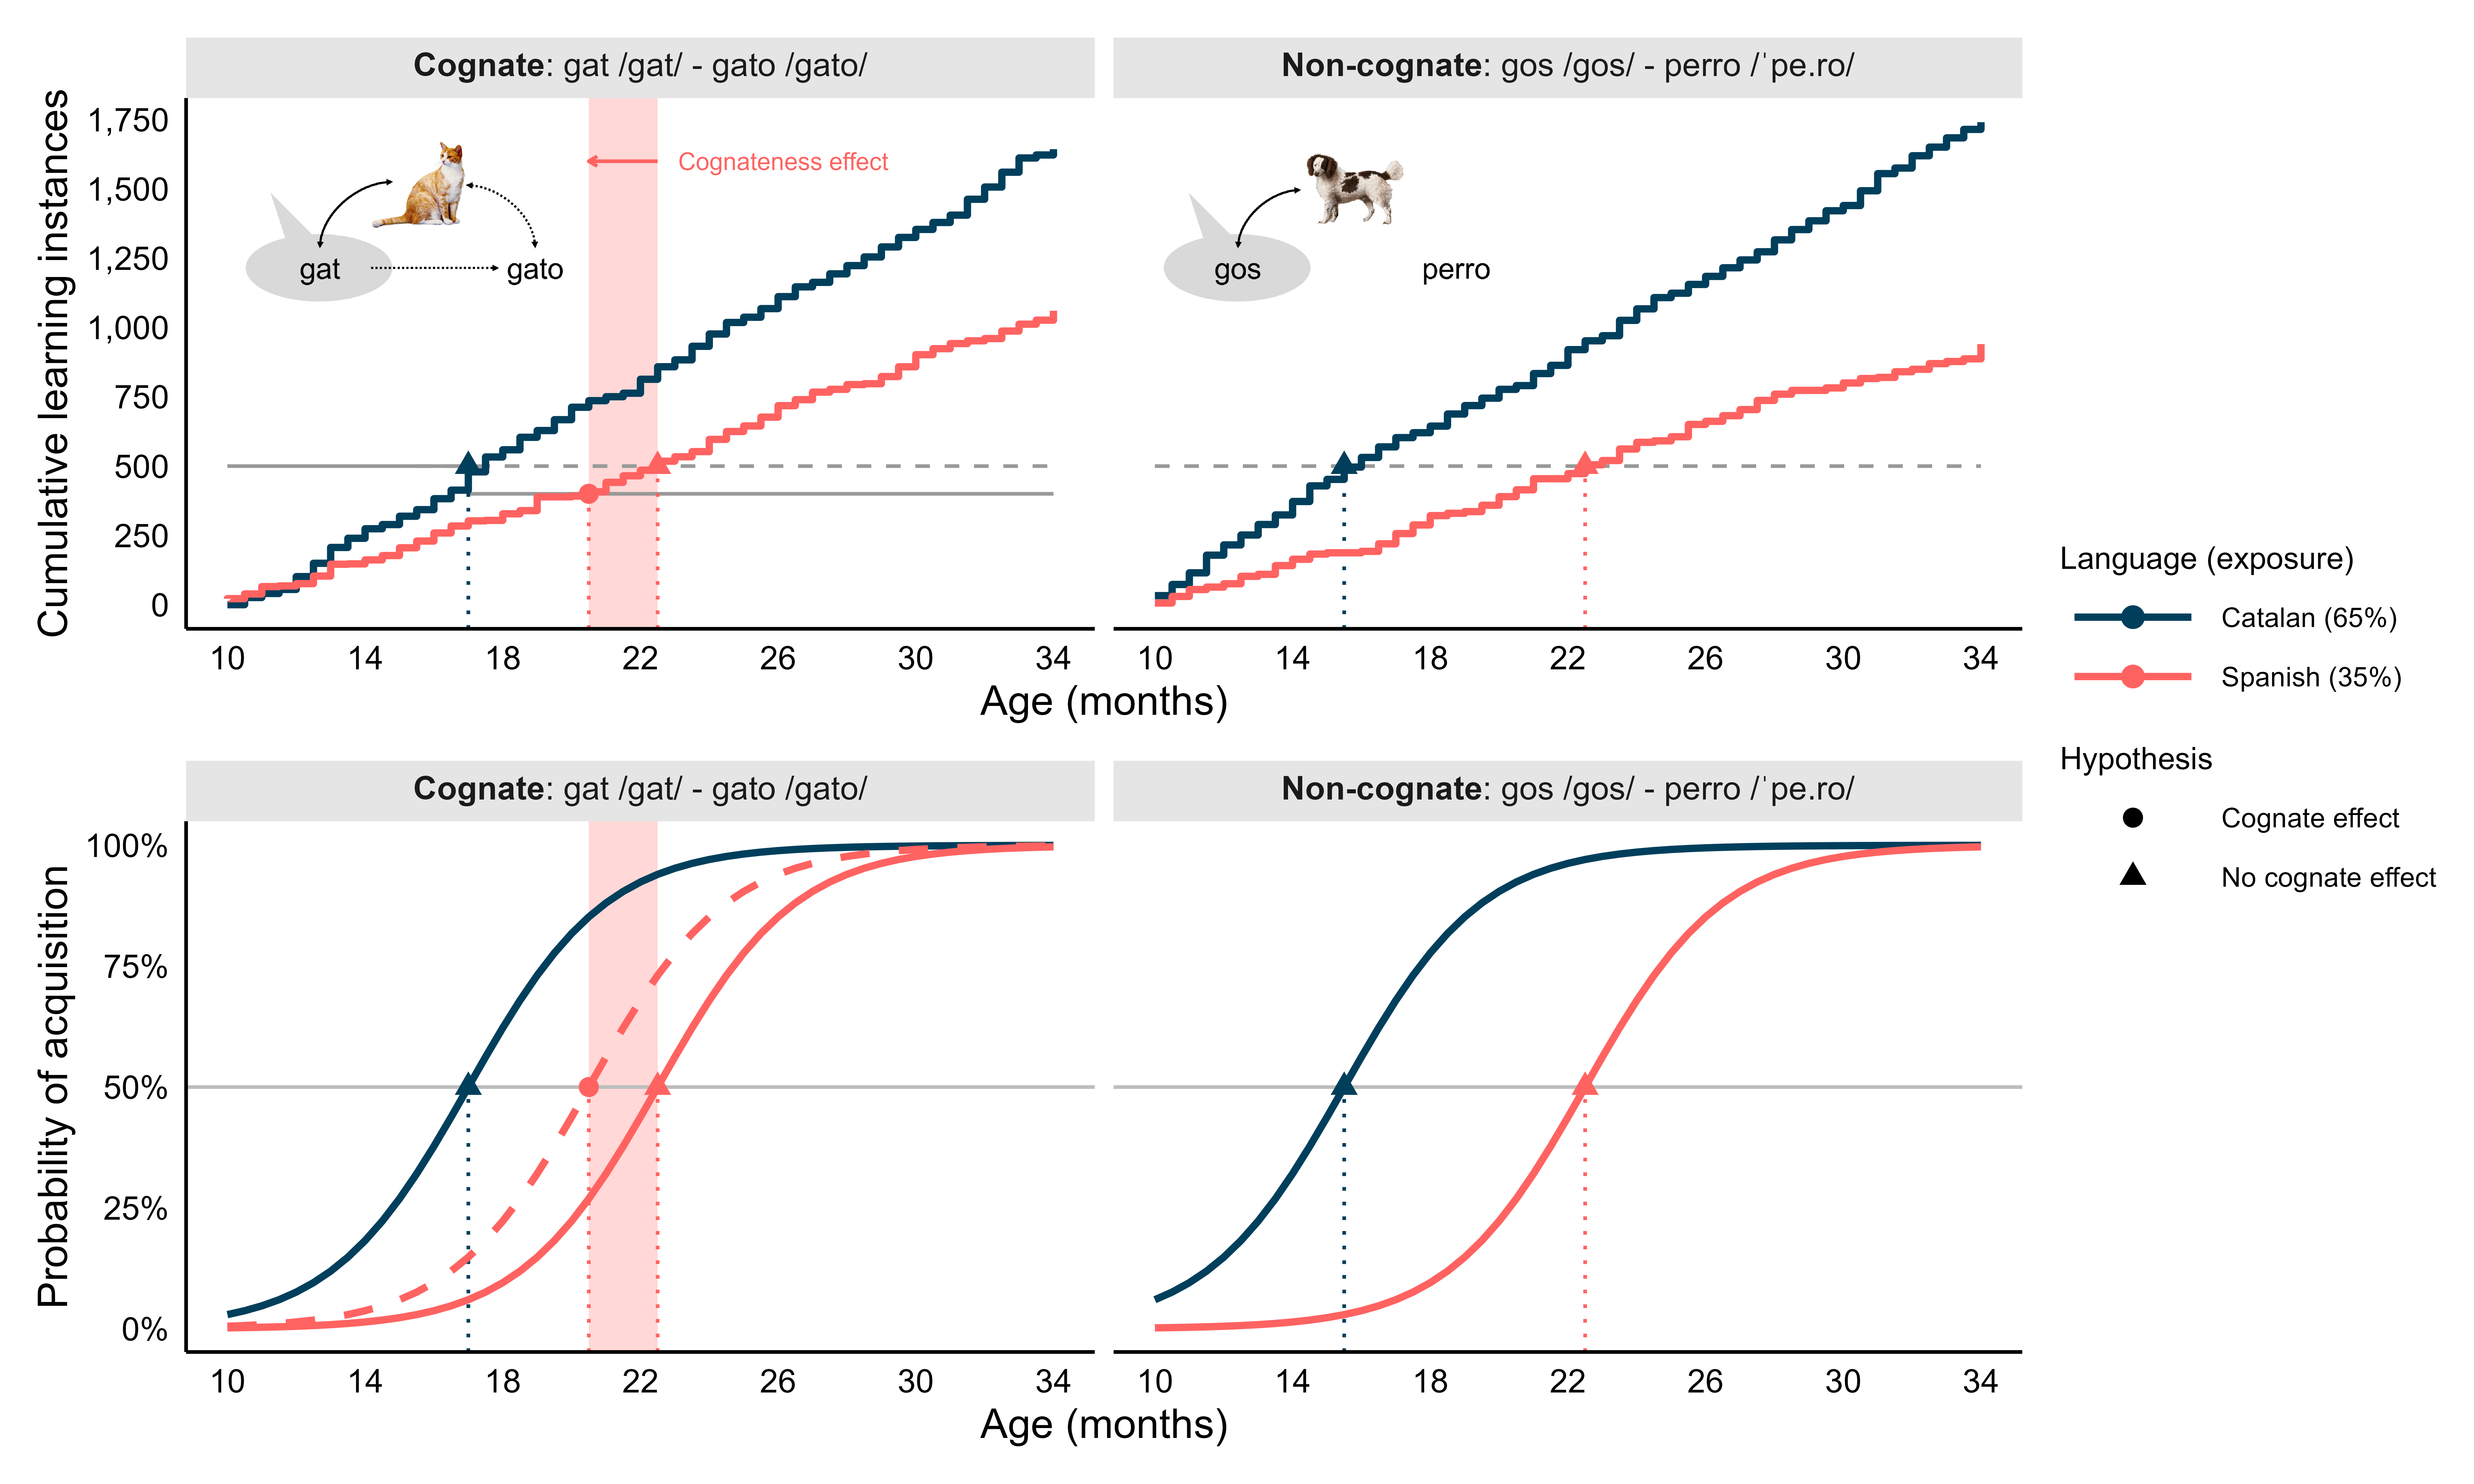
\includegraphics[width=1\linewidth]{assets/img/diagram.png}

\end{figure}

In line with this hypothesis, the size of the effect of linguistic
similarity on vocabulary size that Floccia et al.~reported was larger in
the additional language (language of lower exposure) vocabulary than in
English vocabulary (language of higher exposure). Most participants in
their sample were English-dominant, meaning that their relative amount
of exposure to English was larger than in the additional language.
Therefore, participants may have on average learned the English
word-form of translation equivalents earlier than the word-form in the
additional language. Because of children's imbalance in exposure to
words in English and in the additional language, the acquisition of
English words by English-dominant participants might then benefit less
frequently from their cognate status (the other word-form is unlikely to
be available yet), while the acquisition of words in the additional
language would benefit more frequently from their phonological
similarity with the (more likely available) English translation.

We tested the hypothesis that the cognate effect on word acquisition is
conditional to a child's exposure rate to the word, which would support
the hypothesis that cognateness plays a role in the acquisition of a
word \emph{only} once its translation has been already acquired. We
collected vocabulary data on production and comprehension from a large
sample of bilingual Catalan-Spanish children using an online vocabulary
checklist designed for the present study. Participants were aged 12 to
31 months, and were exposed to Catalan and/or Spanish to varying
degrees. We adopted a Bayesian explanatory item response theory (IRT,
see Kachergis et al., 2022 for a similar approach) approach to model the
probability of a given participant being reported to \emph{understand}
or \emph{understand and say} each word-form in the checklist,
conditional to participants age and rate of exposure to the word-form,
and the cognate status of the word form, while adjusting for the the
number of phonemes in the word form (an indicator of word acquisition
difficulty).

To operationalise participants' exposure rate to a word-form, we used a
composite measure that captures the lexical frequency of the word-form
(an approximation of how often a participant is exposed to it), and
child's amount of exposure to the language such word belongs to. This
measure was calculated by multiplying the word-form's lexical frequency
with participant's degree of exposure to the language the word belongs
to. Lexical frequencies were extracted from the CHILDES corpora
(MacWhinney, 2000; Sanchez et al., 2019) (see Appendix A for more
details). Participants' degree of exposure were reported by caregivers
in a language exposure questionnaire they filled before the vocabulary
checklist. Caregivers provided a proportion of the time the child was
estimated to listen to any language they were spoken to regularly
(described in the methods section). The resulting measure is a
exposure-weighted lexical frequency measure, which was included in
analyses as a proxy of how often bilingual participants were exposed to
each word-form.

\emph{Cognateness} was defined as a continuous measure of phonological
similarity between translation equivalents. We quantified the
phonological similarity between each pair of Catalan-Spanish word-forms
by computing the inverse of the normalised Levenshtein distance between
their X-SAMPA phonetic transcriptions (Levenshtein, 1966; Wells, 1995).
This score is computed by counting the number of insertions, deletions
and replacements needed by both transcriptions to become identical,
dividing the resulting value by the length of the longest transcription,
and finally subtracting this value from one. This results in a
proportion that indicates how much the two phonetic transcriptions of
the translation equivalent are similar to each other, ranging from zero
(no similarity at all) to one (both transcriptions are identical) (see
Floccia, Sambrook, Delle Luche, et al., 2018; Fourtassi et al., 2020;
Laing, 2022 for similar approaches). For instance, this measure of
phonological similarity returns 0\% for \emph{ocell} \texttt{{[}uceL{]}}
and \emph{pájaro} \texttt{{[}paxa4o{]}}, Catalan and Spanish for `bird',
and returns 50\% for \emph{lluna} \texttt{{[}Lun5{]}} and \emph{luna}
\texttt{{[}luna{]}}, Catalan and Spanish for `moon' (see Appendix A for
more details).

\hypertarget{sec-methods}{%
\section{Methods}\label{sec-methods}}

All materials, data, and reproducible code can be found at the OSF
(\url{https://osf.io/hy984/}) and GitHub
(\url{https://github.com/gongcastro/trajectories}) repositories. This
study was conducted according to guidelines laid down in the Declaration
of Helsinki, and was approved by the Drug Research Ethical Committee
(CEIm) of the IMIM Parc de Salut Mar, reference 2020/9080/I.

\hypertarget{sec-questionnaire}{%
\subsection{Questionnaire}\label{sec-questionnaire}}

To collect vocabulary data from participants, we created an \emph{ad
hoc} questionnaire: the Barcelona Vocabulary Questionnaire. This
questionnaire was inspired by the MacArthur-Bates Communicative
Development Inventory (Fenson et al., 2007) and its adaptations to other
languages, and was implemented on-line using the formR platform (Arslan
et al., 2020). This questionnaire is structured in three blocks: (1) a
language exposure questionnaire, (2) a demographic survey, and (3) two
vocabulary checklists. Vocabulary checklists followed a similar
structure as the Oxford Communicative Developmental Inventory (Hamilton
et al., 2000) and consisted in two lists of words: one in Catalan and
one in Spanish. both lists included items from a diverse sample of 26
semantic/functional categories. The Catalan checklist contained 793
items and the Spanish checklist contained 797. Items in one language
were translation equivalents of the items in the other language, roughly
following a one-to-one mapping (e.g., the same participant responded to
both \emph{gos} and \emph{perro}, Catalan and Spanish for `dog') (see
Table~\ref{apatb-items} for a summary of the questionnaire items).

\begin{table}
\caption{Summary of the items included in the final analyses.}
\label{apatb-items}

\begin{longtable*}{l|rrrrrc}
\toprule
\multicolumn{1}{l}{} & List A & List B & List C & List D & Total & Examples \\ 
\midrule
Household items & 31 & 26 & 30 & 25 & 112 & bottle, bed \\ 
Food and drink & 29 & 26 & 23 & 27 & 105 & water (beverage), sandwich \\ 
Animals & 26 & 23 & 19 & 25 & 93 & bee, owl \\ 
Outside & 14 & 13 & 13 & 15 & 55 & tree, ground \\ 
Body parts & 14 & 12 & 11 & 11 & 48 & tummy, mouth \\ 
Toys & 11 & 11 & 12 & 13 & 47 & box, balloon \\ 
Clothes & 12 & 12 & 10 & 10 & 44 & bib, button \\ 
Vehicles & 9 & 10 & 11 & 10 & 40 & airplane, boat \\ 
Colours & 6 & 6 & 6 & 6 & 24 & yellow, blue \\ 
People & 7 & 4 & 6 & 6 & 23 & child, grandma \\ 
Furniture and rooms & 4 & 4 & 4 & 4 & 16 & bath, kitchen \\ 
Time & 2 & 2 & 2 & 2 & 8 & day, night \\ 
Adventures & 1 & 1 & 1 & 1 & 4 & witch \\ 
Parts of things & 1 & 1 & 1 & 1 & 4 & wheel \\ 
\bottomrule
\end{longtable*}

\end{table}

For each word included in the vocabulary checklists, we asked parents to
report whether their child was able to understand it, understand
\emph{and} say it, or did not understand or say it (checked out by
default). Given the large number of words in the vocabulary checklists,
we created four different subsets of the complete list of items. Each
subset contained a random but representative sub-sample of the items
from the complete list. Semantic/functional categories with less than 16
items---thus resulting in less than four items after dividing it in four
lists---were not divided in the short version of the questionnaire: all
of their items were included in the four lists. Items that were part of
the trial lists of some ongoing experiments in the lab were also
included in all versions. The resulting reduced vocabulary checklists
contained between 343 and 349 Catalan words, and between 349 and 371
Spanish words. Participants were randomly allocated into one of the four
subsets. Each response to the questionnaire provided data for a minimum
of 343 and a maximum of 371 translation equivalents.

\hypertarget{sec-participants}{%
\subsection{Participants}\label{sec-participants}}

We collected 436 responses to the questionnaire from 367 distinct
children from the Metropolitan Area of Barcelona between the 30th of
March, 2020 and the 31th of October, 2022: 314 of those participants
participated once, 41 twice, 8 three times, and 4 four times. Recurrent
participants provided responses with a minimum of 25 days between
responses, and a maximum of 527, and were always allocated to the same
questionnaire list (A, B, C, or D). Participants were part of the
database of the Laboratori de Recerca en Infància (Universitat Pompeu
Fabra), and were contacted by e-mail or phone if their child were aged
between 12 and 32 months, and had not been reported to be exposed more
than 10\% of the time to a language other than Spanish or Catalan (see
Table~\ref{apatb-participants} for a more detailed description of the
sample). In total, 70 participants (16.06\%) participants were reported
to be exposed to a third language other than Catalan and Spanish. All
families provided informed consent before participating. Upon consent,
families were sent a link to the questionnaire via e-mail, which they
filled from a computer, laptop, or mobile device. Filling the
questionnaire took 30 minutes approximately. After completion, families
were rewarded with a token of appreciation.

\begin{table}
\caption{Participant sample size by age and degree of exposure to Catalan.}
\label{apatb-participants}

\begin{longtable*}{l|rrrrrrr}
\toprule
\multicolumn{1}{l}{} &  & \multicolumn{6}{c}{Age (months)} \\ 
\cmidrule(lr){3-8}
\multicolumn{1}{l}{} & Catalan exposure & [10,14] & (14,18] & (18,22] & (22,26] & (26,30] & (30,34] \\ 
\midrule
 & 75-100\% & 17 & 23 & 36 & 39 & 20 & 6 \\ 
 & 50-75\% & 8 & 13 & 27 & 38 & 21 & 1 \\ 
 & 25-50\% & 10 & 16 & 48 & 28 & 20 & – \\ 
 & 0-25\% & 6 & 12 & 21 & 16 & 9 & 1 \\ 
\midrule 
\midrule 
Total & — & $41$ & $64$ & $132$ & $121$ & $70$ & $8$ \\ 
\bottomrule
\end{longtable*}

\tablenote{Information about language degree of exposure (DoE) was provided by families before filling the questionnaire. In this table, a 100\% indicates that the participant was exclusively exposed to Catalan, and never to Spanish. A 0\% indicates that the participant was not exposed to Catalan ever, and most of the time to Spanish. A 50\% indicates that the participant was exposed to Catalan and Spanish approximately half of the time each. The 100\%, 0\%, and 50\% would be traditionaly classified as Catalan monolingual, Spanish monolingual, and Catalan-Spanish bilingual, respectively. For illustration purposes this table, DoEs were binned into 25\%-wide bins, and ages (in months) binned into 4 month-wide bins. Hyphens indicate that no participants from that specific combination of age and DoE filled the questionnaire.}

\end{table}

We used the highest self-reported educational attainment of parents or
caregivers as a proxy of participants' socio-economic status (SES). This
information was provided by each parent or caregiver by selecting one of
six possible alternatives in line with the current educational system in
Spain: `sense escolaritzar/sin escolarizar' {[}no education{]},
`educació primària/educación primaria' {[}primary school{]}, `educació
secundària/educación secundaria' {[}secondary school{]},
`batxillerat/bachillerato' {[}complementary studies/high school{]},
`cicles formatius/ciclos formativos' {[}vocational training{]}, and
`educació universitària/educación universitaria' {[}university
degree{]}. Most families reported university studies (355, 82\%),
followed by families were the highest educational attainment were
vocational studies (61, 14\%), complementary studies (6, 1\%), secondary
education (8, 2\%), no formal education (2, \textless1\%) and primary
education (1, \textless1\%).

\hypertarget{sec-analysis}{%
\subsection{Data analysis}\label{sec-analysis}}

From the responses to the 1,590 items included in the questionnaire, we
restricted the analyses to responses to nouns (628 items corresponding
to other grammatical classes were excluded) (Fourtassi et al., 2020). We
then excluded items with missing lexical frequency scores (\emph{n} =
269), items that included more than one lemma (e.g., \emph{mono/mico}
{[}monkey{]}, \emph{n} = 48), multi-word items or phrases (e.g.,
\emph{barrita de cereales} {[}cereal bar{]}, \emph{n} = 9). Finally, we
removed items without a translation in the other language (\emph{n} =
32). This resulted in a final list of 604 items, corresponding to words
302 Catalan words and their 302 Spanish translations (302 translation
equivalents). After collecting participants' responses, the final
dataset consisted of 138,050 observations, each corresponding to a
single response of one participant to one item. Each translation
equivalent received a median of 232 responses (\emph{Min} = 106,
\emph{Max} = 872) from participants, both languages pooled together.

We modelled the probability of participants answering each response
category (\emph{No} \textless{} \emph{Understands} \textless{}
\emph{Understands and Says}) using a Bayesian, mixed-effects ordinal
regression model (4 sampling chains with 1,000 iterations each). This
model allowed us to estimate both item and participant word-acquisition
trajectories, as a function of different fixed effects from
\(\text{Age}\) (number of months elapsed between participants' birth
date and questionnaire completion), \(\text{Length}\) (number of
phonemes in the X-SAMPA phonological transcription of the word-form),
\(\text{Exposure}\) (composite measure of lexical frequency and language
degree of exposure), and \(\text{Cognateness}\) (a measure of
cognateness, defined as the phonological similarity between translation
equivalents). For an easier interpretation of the regression
coefficients, the values of all predictors were standardised before
entering the model by subtracting the mean of the predictor from each
value and dividing the result by the standard deviation of the
predictor. Participant- and item-level random intercepts and slopes were
included when appropriate, according to the structure of the data (Barr
et al., 2013). We specified a weakly informative prior around the
parameters of the model (see Appendix C for details).

We built a baseline model \(\mathcal{M}_{0}\) that only included the
intercept and the main effects of \(\text{Age}\), \(\text{Length}\), and
\(\text{Exposure}\) as predictors, and compared it against increasingly
more complex models, which introduced predictors in the following order:
\(\text{Age} \times \text{Exposure}\) (\(\mathcal{M}_{1}\)),
\(\text{Cognateness}\) (\(\mathcal{M}_{2}\)),
\(\text{Exposure} \times \text{Cognateness}\) (\(\mathcal{M}_{3}\)), and
finally \(\text{Age} \times \text{Cognateness}\) and
\(\text{Age} \times \text{Exposure} \times \text{Cognateness}\)
(\(\mathcal{M}_{4}\)). We compared the predictive performance of the
models using Bayesian leave-one-out cross-validation (LOO-CV, Vehtari et
al., 2017)\footnote{Due to computational constraints, we performed
  LOO-CV based on a random sub-sample of 700 samples of the posterior
  distribution of the fixed effects (Magnusson et al., 2020)}. LOO-CV
involves computing the likelihood of each data point, given a model
fitted excluding such data point. The likelihoods generated by the model
for each of the data points are summarised together in a measure of
predictive performance: the expected log-predicted density (ELPD). This
measure penalises the complexity of the model ELPD. ELPD values closer
to zero indicate better predictive accuracy. We compared the ELPD of
each model, and selected for interpretation the one showing the best
performance (see Appendix C for more details about the models).

We assessed the practical relevance of the estimated regression
coefficients of the selected model following Kruschke and Liddell
(2018). First, we specified a region of practical equivalence (ROPE)
from -2.5\% to +2.5\%, in the probability scale. This region indicates
the range of values that we considered equivalent to zero. The degree of
overlap between the posterior distribution of a regression coefficient
with the can be interpreted as support for the true parameter of the
coefficient being zero or equivalent. We then computed the 95\% highest
density interval (HDI) of the posterior distribution of each regression
coefficient. This interval contains the true value of this coefficient
with 95\% probability, given the data. Finally, we calculated the
proportion of posterior samples in the 95\% HDI that fell into the ROPE,
which indicates the probability that the true value of the regression
coefficient falls into the ROPE, and should therefore be considered
equivalent to zero. For example, a 90\% overlap between the HDI of a
coefficient's posterior distribution and the indicates that, given our
data, there is a 90\% probability that the true value of the coefficient
falls within the ROPE, and is therefore equivalent to zero.

Data processing and visualisation was done in R (R Core Team, 2013,
version 4.2.2) using the Tidyverse family of packages (Wickham et al.,
2019). Bayesian modelling was done using the \texttt{brms} (Bürkner,
2017; Carpenter et al., 2017), \texttt{loo} (Vehtari et al., 2022),
\texttt{tidybayes} (Kay, 2021) and \texttt{marginaleffects}
(Arel-Bundock, 2022) R packages.

\hypertarget{sec-results}{%
\section{Results}\label{sec-results}}

All models showed adequate convergence diagnostics and little evidence
of multicollinearity between predictors (see Appendix D for details).
\(\mathcal{M}_{3}\), which did \emph{not} include the
\(\text{Age} \times \text{Exposure} \times \text{Cognateness}\)
three-way interaction, showed the best predictive performance with a
difference in expected log-predicted density (ELPD) compared to the
second best-performing model (\(\mathcal{M}_{4}\)) of -109.17 \(\pm\)
40.05. Given our data, the predictions of the \(\mathcal{M}_{3}\) are
confidently more accurate than those of the other models (see
Table~\ref{apatb-results-loos} for all model comparisons). Both
\(\mathcal{M}_3\) and \(\mathcal{M}_4\) performed considerably better
than the rest of the models, which did not include the
\(\text{Exposure} \times \text{Cognateness}\) two-way interaction. This
points to the effect of \(\text{Cognateness}\) being strongly modulated
by \(\text{Exposure}\), and that this interaction remains relatively
stable across ages.

\begin{table}
\caption{Bayesian leave-one-out cross validation (LOO-CV).}
\label{apatb-results-loos}

\begin{longtable*}{l|rr}
\toprule
\multicolumn{1}{l}{} & ELPD \$\$\textbackslash{}pm\$\$ SE & Diff. \$\$\textbackslash{}pm\$\$ SE \\ 
\midrule
Model 3 & $-142,586.09$ ± $317.78$ & $0.00$ ± $0.00$ \\ 
Model 4 & $-142,695.26$ ± $319.90$ & $-109.17$ ± $40.05$ \\ 
Model 1 & $-143,112.89$ ± $315.28$ & $-526.80$ ± $63.02$ \\ 
Model 2 & $-143,152.04$ ± $321.28$ & $-565.95$ ± $33.74$ \\ 
Model 0 & $-144,709.07$ ± $317.31$ & $-2,122.98$ ± $83.59$ \\ 
\bottomrule
\end{longtable*}

\tablenote{We report the ELPD of each model along their associated standard errors (SE). The last column indicates the difference in ELPD between each model and the model with the best predictive accuracy (Model 3). Pareto-k estimates of all models were acceptable (k < 0.5).}

\end{table}

Table~\ref{apatb-coefs} shows the summary of the posterior distribution
of the fixed regression coefficients of \(\mathcal{M}_{3}\), and their
degree of overlap with the ROPE. For interpretability, we report the
estimated regression coefficients transformed to the probability scale.
The resulting values correspond to the maximum difference in probability
of acquisition (\emph{Comprehension} or \emph{Comprehension and
Production}) that corresponds to a one standard deviation change in each
predictor\footnote{The logit and probability scales relate non-linearly.
  This means that one logit difference is not necessarily translated to
  a unique value in the probability scale. For example, the probability
  of acquisition of a given word might increase in 5\% when age
  increases from 22 to 23 months, the probability of acquisition of the
  same word might only increase in 0.2\% when age increases from 30 to
  32 months. The linear growth of the probability of acquisition differs
  along the logistic curve, and therefore deciding the age point at
  which to report the estimates of the regression coefficients in the
  probability scale is not trivial. Following Gelman et al. (2020), we
  report the maximum value of such coefficient, which corresponds to the
  linear growth (i.e.~derivative) of the logistic curve at the age at
  which most participants were acquiring a given word. This value can be
  approximated by dividing the coefficient in the logit scale by four:
  \(\hat{\beta_j}/4\), where \(\hat{\beta_j}\) is the estimated mean of
  the posterior distribution of coefficient \(j\).}.

\begin{table}
\caption{Posterior distribution of regression coefficients Model 3.}
\label{apatb-coefs}

\begin{longtable*}{l|rrr}
\toprule
\multicolumn{1}{l}{} & Median & 95\% HDI & ROPE prob. \\ 
\midrule
\multicolumn{4}{l}{Intercepts (at 22 months)} \\ 
\midrule
Comprehension and Production & $0.21$ & [$0.19$, $0.23$] & $0.00\%$ \\ 
Comprehension & $0.84$ & [$0.82$, $0.85$] & $0.00\%$ \\ 
\midrule
\multicolumn{4}{l}{Slopes} \\ 
\midrule
Age (+1 SD, 4.81, months) & $0.39$ & [$0.34$, $0.44$] & $0.00\%$ \\ 
Exposure (+1 SD, 1.81) & $0.20$ & [$0.17$, $0.23$] & $0.00\%$ \\ 
Length (+1 SD, 1.56 phonemes) & $-0.08$ & [$-0.10$, $-0.05$] & $0.00\%$ \\ 
Cognateness (+1 SD, 26\%) & $0.06$ & [$0.02$, $0.10$] & $0.42\%$ \\ 
Age × Exposure & $0.06$ & [$0.03$, $0.10$] & $0.00\%$ \\ 
Exposure × Cognateness & $-0.04$ & [$-0.05$, $-0.03$] & $0.00\%$ \\ 
\bottomrule
\end{longtable*}

\tablenote{Median: median of the posterior distribution in the probability scale. 95\% HDI: 95\% highest density interval of the distribution; narrowest range of values that contains 95\% of the distribution, and therefore is 95\% likely to contain the true value, given the data. On top of each distribution, we indicate the proportion of posterior samples in the 95\% HDI that fall into the region of practical equivalence (ROPE). This proportion indicates the probability of the true value of the coefficient being equivalent to zero. Lower values indicate that the true value is unlikely to be zero of equivalent to zero.}

\end{table}

The main effect of \(\text{Age}\) showed the strongest association with
the probability of acquisition (\(\beta\) = 0.39, 95\% HDI = {[}0.34,
0.44{]}), with all of its posterior samples falling out of the ROPE. A
one-month increment in age increased a maximum of 0.08 the probability
of acquisition. Similarly, the word exposure index (\(\text{Exposure}\))
had a strong effect on the probability of acquisition (\(\beta\) = 0.2,
95\% HDI = {[}0.17, 0.23{]}). All of the posterior samples of this
regression coefficient excluded the ROPE. The impact of this predictor
on the probability of acquisition was positive: for every standard
deviation increase in exposure, the participant was 0.11 more likely to
acquire it. Word-form length also showed a significant association with
probability of acquisition (\(\beta\) = -0.08, 95\% HDI = {[}-0.1,
-0.05{]}). For every phoneme in the word-form, participants were -0.05
less likely to know it. The 95\% HDI of the regression coefficient of
the \(\text{Age} \times \text{Exposure}\) interaction also excluded the
ROPE (\(\beta\) = 0.06, 95\% HDI = {[}0.03, 0.1{]}), showing that the
effect of the word exposure index differed across ages: older children
were more sensitive likely to acquire words with higher exposure rate
than younger children.

The posterior distribution of the main effect of cognateness excluded
the ROPE completely (\(\beta\) = 0.06, 95\% HDI = {[}0.02, 0.1{]}). For
every 10\% increment in cognateness, the acquisition of a word increased
in 0.01. The effect of \(\text{Cognateness}\) interacted with that of
\(\text{Exposure}\): the 95\% HDI of the regression coefficient of
interaction excluded the ROPE entirely (\(\beta\) = -0.04, 95\% HDI =
{[}-0.05, -0.03{]}), suggesting that the effect of cognateness on a
word's probability of acquisition changed depending on participants'
exposure to word. Follow-up analyses on this interaction showed that
when exposure rate was low (e.g., -1 SD), cognateness increased the
probability of acquisition substantially. This effect was negligible
when for words with median or high exposure (+1 SD) (see
Figure~\ref{apafg-results-marginal}).

\begin{figure}[h!]
\caption{Posterior marginal effects of Model 3. Thin lines correspond to 50 mean predictions generated from 50 MCMC samples of the posterior distribution of the model. Thicker lines indicate the median of those predictions. Different colours indicate different levels of phonological similarity (as indicated by the Cognateness similarity between pairs of translation equivalents). Predictions are presented separately for different degrees of word exposure index: little exposure to the word, mean exposure, and high exposure. Predictions for Comprehension are show on top and predictions for Comprehension and Production are shown on the bottom. In-sample predictions lie inside the grey rectangles.}
\label{apafg-results-marginal}
\includegraphics[width=8 in]{manuscript_files/figure-pdf/apafg-results-marginal-1.pdf}

\end{figure}

\hypertarget{sec-discussion}{%
\section{Discussion}\label{sec-discussion}}

The present study explored the cognateness facilitation effect on
bilingual word acquisition. We found such effect to be mediated by
lexical frequency and degree of language exposure: phonologically
similar translation equivalents were on average acquired earlier in age
compared to phonologically dissimilar translation equivalents, but this
effect was only observed for word-forms to which participants were
exposed less often, i.e., words with low lexical frequency and/or words
from the language of lower daily exposure. Our results are relevant in
the light of two previous findings. First, Floccia, Sambrook, Delle
Luche, et al. (2018) reported that bilingual toddlers learning two
typologically close languages (which shared many cognates, e.g.,
English-German) showed larger vocabulary sizes than those learning
typologically more distance languages (which shared fewer cognates,
e.g., English-Mandarin). Second, Mitchell et al. (2022) found an earlier
age-of-acquisition for cognates, compared to non-cognates. The outcomes
of both studies pointed to cognateness facilitating word acquisition,
but the underpinnings of such effect were unclear.

In this study, we capitalised on accumulator models of language
acquisition to propose a theoretical account of bilingual word learning,
in which cognateness interacts with lexical frequency and language
exposure to boost the acquisition of translation equivalents. We
suggested that words benefit from their cognate status only \emph{after}
their translation equivalent has been acquired: after the child acquires
a word-form, the number of learning instances they need to acquire its
translation decreases. We further hypothesised that such facilitation is
proportional to the phonological similarity between both word-forms. If
two translation equivalents sharing a fair deal of phonological
similarity (e.g., /\textipa{"pOR.t@}/-/\textipa{"pweR.ta}/, 50\%
Levenshtein similarity), learning of one of them should facilitate the
acquisition of the other more strongly, compared to when both word-forms
share only few phonemes (e.g.,
/\textipa{k@"Di.R@}/-/\textipa{"si.\textlambda a}/ , 25\%).

Under such scenario, we predicted that words from the language of lower
exposure would benefit more often from their cognate status than those
from the language of higher exposure. The rationale behind such
prediction was that children are less frequently exposed to word-forms
in the former language than to words in the latter (Cattani et al.,
2014; Thordardottir et al., 2006). Words in the language of lower
exposure are therefore more likely to be acquired later in age than
their translations in the other language. For instance, an infant
exposed to Catalan and Spanish 65\% and 35\% of the time, respectively,
is more likely to learn the Spanish word-form /\textipa{"ga.to}/ later
in age than its Catalan translation /\textipa{gat}/. If this is the
case, /\textipa{"ga.to}/ is more likely to receive facilitation from the
acquisition of /\textipa{gat}/ than \emph{vice versa} (see
Figure~\ref{apafg-hypotheses} for a graphic illustration). In line with
these predictions, we found that cognateness facilitated word
acquisition more strongly in words from the language of lower exposure.
This asymmetric facilitation effect provides support for the hypothesis
that words benefit from their cognate status \emph{after} their
translation has been acquired. Overall, our results provide support for
an interactive account of bilingual vocabulary learning in which word
representations from one language contribute to the acquisition of words
in the other.

These findings are, to a large extent, in line with previous literature
on word acquisition. First, words-forms with fewer phonemes like
/\textipa{sO\textltilde}/ (Catalan for \emph{sun}) were on average more
likely to be acquired than word-forms with more phonemes like
/\textipa{ku.ku"DRi\textltilde}/ (Catalan for \emph{crocodile}). These
results converge with previous studies found word length to be more
strongly associated with receptive vocabulary than with expressive
vocabulary (e.g., Braginsky et al., 2019; Jones \& Brandt, 2019). This
facilitation is most likely due to the fact that shorter word-forms are
generally simpler to encode as phonological representations in the
lexicon than longer word-forms. Shorter word-forms are easier to
produce, and therefore to be reported as acquired in parental vocabulary
checklists.

Our participants were also more likely to know words to which they were
more frequently exposed to, replicating previously reported effects of
lexical frequency (e.g., Braginsky et al., 2019), and bilingual language
exposure (e.g., Cattani et al., 2014; Thordardottir et al., 2006). This
strong effect of word frequency is a key component of accumulator models
of word acquisition, which suggest that the age-of-acquisition of a word
is, to a large extent, a function of the child's rate of exposure to
such word, which conspires with child- and word-level factors in the
process of forming a representation of the word in the child's lexicon
(Hidaka, 2013; Mollica \& Piantadosi, 2017). Our results provide ground
for the central role of word frequency in accumulator models to be
extended to the bilingual case, in the form of a composite measure of
word rate of exposure that accounted for both lexical frequency and
language exposure (Cattani et al., 2014; Floccia, Sambrook, Luche, et
al., 2018b). Interestingly, our findings pointed to this predictor
playing a stronger role during earlier ages: younger infants benefited
from higher exposure rates at earlier ages, suggesting that early word
acquisition is supported by mere exposure to word forms more strongly
than later word acquisition.

Finally, we found a frequency-mediated facilitation effect of
cognateness, adding some nuance to the findings from previous studies
(Bosch \& Ramon-Casas, 2014; Floccia, Sambrook, Luche, et al., 2018b;
Mitchell et al., 2022; Schelletter, 2002). Only words to which children
were exposed to less frequently benefited from their cognate status.
These results favour the account that a word-form benefits from its
phonological similarity with its translation only after such translation
has been acquired first. On the one hand, our results provide converging
evidence for Floccia, Sambrook, Luche, et al. (2018b), and arguably
account for the language distance facilitation effect they found in the
additional (non-English) language of their bilingual sample. Most
children in their sample were English-dominant, and therefore their
exposure to English was higher than their exposure to the additional
language. However, it was in the vocabulary of the additional language
where the authors found a facilitation effect of cognateness: bilingual
children learning two languages that shared many cognateness (e.g.,
English-German) had larger vocabularies in their additional language
than those bilingual who were learning two languages that shared less
cognates (e.g., English-Chinese). Given our results, we argue that it is
language exposure that mediates the relationship between cognateness and
vocabulary size in Floccia, Sambrook, Luche, et al. (2018b)'s sample.

Overall, our findings parallel cognates' significant role in many models
of bilingual language processing. The importance of cognates in these
model stems in the fact that cognates provide evidence for a language
non-selective account of lexical processing, in which bilinguals
activate unselected lexical representations in both languages, even in
fully monolingual situations (Christoffels et al., 2007; Thierry \& Wu,
2007). As mentioned in the introduction, naming pictures whose labels
are cognates leads to shorter latencies than when labels are
non-cognates, which suggests that phonological similarity across
translations facilitates production (Costa et al., 2000; Hoshino \&
Kroll, 2008). When acting as distractors in naming tasks, cognates exert
larger interference effects than non-cognate distractors (Colomé \&
Miozzo, 2010; Hoshino \& Thierry, 2011). Both findings suggest that the
non-selected translation of the target in Costa et al. (2000), or of the
distractor in Colomé and Miozzo (2010) was activated, and that when such
word-form was phonologically related to its translation, the
facilitation or interference effect was stronger.

Evidence supporting the language-non selective account of lexical access
is not restricted to production or the auditory modality, but rather
extend to comprehension and translation, and to the visual modality
(reading and signing) (Gimeno-Martínez et al., 2021; Hell \& Groot,
2008; Morford et al., 2011; Schwartz et al., 2007; Schwartz \& Kroll,
2006; Spivey \& Marian, 1999; see Kroll et al., 2013 for review). For
instance, Thierry and Wu (2007) found neurophysiological evidence of
Chinese-English bilinguals activating both languages in a word
comprehension task. In this experiment, participants were presented with
couples of words in English, and were asked to respond if the words were
related in meaning. Unbeknownst to participants, the translations to
Chinese of half of such word pairs shared a character. Participants
would be presented (visually in a first experiment and auditorily in a
second experiment) with an English word pair `train-ham', which are
semantically unrelated, but share a character in their Chinese
translations (\foreignlanguage{chinese-simplified}{火車} {[}Huo
Che{]}-\foreignlanguage{chinese-simplified}{火腿} {[}Huo Tui{]}).
Bilinguals' brain signal differed across words pairs with and without
translation overlap (e.g., `apple-table',
\foreignlanguage{chinese-simplified}{平果} {[}Ping
Guo{]}--\foreignlanguage{chinese-simplified}{桌子} {[}Zhuo Zi{]}). This
suggests that participants were sensitive to the form-similarity of the
Chinese translation of the word-pairs they were presented, despite the
whole experimental task taking place in English.

Bilingual toddlers and children---still in the process to developing a
mature lexicon---also show evidence of parallel activation during
comprehension (Bosma \& Nota, 2020; Poarch \& Hell, 2012; Schröter \&
Schroeder, 2016; Von Holzen et al., 2019; Von Holzen \& Mani, 2012).
Whether---and if so, how---the language non-selectivity shapes the early
bilingual lexicon is still unclear. Previous work has pointed to an
interactive account of lexical acquisition, in which toddlers' lexical
representations in one language influence the acquisition of words in
the other language. The acquisition of translation equivalents embodies
a notable divergence between monolingual and bilingual developmental
trajectories. For instance, monolingual word acquisition benefits from
the semantic relatedness between the words the child learns (Fourtassi
et al., 2020; Hills et al., 2009), but is inhibited during the
acquisition of words from the same language with the \emph{equivalent}
meaning, i.e.~synonyms. This learning heuristic, called \emph{mutual
exclusivity}, is one of many that play a relevant role in models of
monolingual word learning (Golinkoff et al., 1994), acting as a
constrainer of the hypothesis space for all possible word-referent
associations: if a referent already holds a label, any label uttered in
the presence of such referent is associated with a different referent
(e.g., Markman, 1990). Although this heuristic seems useful in the
monolingual case (children are rarely exposed to synonyms), it would
come with a huge cost for bilinguals, how are frequently exposed to more
than one label for the same referent, one in each language. It was
initially predicted that bilinguals would follow \emph{mutual
exclusivity}, and therefore avoid learning translation equivalents
(Volterra \& Taeschner, 1978).

This prediction has been robustly contested by two main sources of
evidence. First, experimental work suggests that bilinguals may not
apply \emph{mutual exclusivity} during word learning, or at least not as
consistently monolinguals do (Byers-Heinlein \& Werker, 2009, 2013).
Second, detailed analyses of bilingual children's vocabulary contents
shows that bilingual children do acquire translation equivalents from
early ages (e.g., Pearson et al., 1995). In fact, translation
equivalents may even be overrepresented in the early bilingual lexicon.
For instance, Bilson et al. (2015) found that bilingual toddlers
produced a higher proportion of translation equivalents than it would be
expected if they learned two independent lexica simultaneously, which
suggests that bilingual children preferentially acquired words for which
they already knew a label in the other language. In the same line, Bosch
and Ramon-Casas (2014) reported a similar overrepresentation of
translation equivalents in Catalan-Spanish bilinguals: a high proportion
of acquired Catalan words held an also acquired translation in Spanish.
Finally, a recent investigation by Tsui et al. (2022b) presented a
quantitative model of bilingual vocabulary acquisition which showed a
consistent preferential acquisition of translation equivalents by
English-French bilinguals, with such preference being stronger at early
stages of vocabulary growth. Overall, these findings suggest that
bilingual children benefit from a semantic facilitation effect driven by
the acquisition of translation equivalents. This is a substantial
divergence from monolingual trajectories of lexical acquisition. Our
study provides further evidence for a pivotal role of translation
equivalents, showing that, especially in the case of cognates,
translation equivalents, are not only part of bilinguals' vocabulary
contents, but are also acquired close in age, depending primarily on
children's degree of exposure to each language.

The divergent trajectories of bilingual lexical acquisition go beyond
semantics. As highlighted before, the phonological overlap between the
languages being learned seems to impact vocabulary growth in bilinguals.
Bilinguals learning languages that share many cognates show larger
vocabulary sizes than those learning two languages sharing fewer
cognates (Blom et al., 2020; Bosma et al., 2019; Floccia, Sambrook,
Delle Luche, et al., 2018). This finding can be explained to a large
extent by the fact that cognates seem to be acquired at earlier ages
than non-cognates (Mitchell et al., 2022). This phonological
facilitation effect mimics previous findings in monolinguals, who seem
to preferentially learn phonologically similar words. For instance,
Jones and Brandt (2019) found that English monolingual toddlers show a
facilitation effect when acquiring words from dense phonological
neighbourhoods: a larger number of similar-sounding words was associated
with an increase in likelihood of a word form being part of a toddler's
productive vocabulary. A network analysis by Fourtassi et al. (2020)
found evidence in favour of a phonological (and semantic) preferential
acquisition of new words in monolingual children: words with higher
phonological relatedness to other words were more likely to be acquired.
Again, these findings contrast with those in bilingual children in that
the facilitation effect or preferential acquisition mechanisms described
are based on phonological similarity \emph{without} translation
equivalence. The amount of similar-sounding words in the child input or
their acquired vocabulary predicts a larger probability of acquisition
of new words with \emph{different} meaning. In the case of bilinguals,
there is evidence of such phonological facilitation at the level of
translation equivalents, as shown by an earlier acquisition of cognates
than non-cognates in English-French (Mitchell et al., 2022) and in the
Catalan-Spanish bilinguals in the present study. Evidence of a
cross-language facilitation effect between non-translation equivalents
is to date absent.

We consider three alternative explanations for our results. Regarding
the cognate facilitation effect, it is possible that when hearing
cognate translation equivalents, bilingual children accept both word
forms as acceptable variations of the \emph{same} word. This contrasts
with monolinguals' high sensitivity to mispronunciations during word
recognition (Bailey \& Plunkett, 2002; Mani \& Plunkett, 2011; Swingley,
2005; Swingley \& Aslin, 2000; Tamási et al., 2017). It might be the
case that every exposure to either of the word-forms of the translation
equivalent is counted as a learning instance for both. This would impact
the acquisition mechanism in such way that any cognate effect is not
explained by a reduction of the number of learning instances needed to
acquired a word (after its translation has been acquired), but by a
faster increase in cumulative learning instances across ages, leading to
a similar outcome: an earlier age-of-acquisition for cognates.
Supporting such alternative explanation, Ramon-Casas et al. (2009)
examined 18-26 months-old Catalan-Spanish bilingual toddlers'
sensitivity to mispronunciations in a word-recognition task and found
that, contrary to their Catalan monolingual peers, bilinguals seemed to
recognise mispronounced words, disregarding vowel replacements involving
the Catalan vowel contrast /e/-/\textepsilon/. The same population of
bilingual infants shows sensitivity to such contrast before 12 months of
age in phoneme discrimination tasks (Bosch \& Sebastián-Gallés,
2003)---which do not involve word-referent associations---suggesting
that bilingual infants dismiss subtle changes in phonological forms when
presented with their referents. Using the same procedure, Ramon-Casas
and Bosch (2010) tested bilingual infants' recognition of
mispronunciations involving the /e/-/\textepsilon/ contrast embedded in
exclusively \emph{non-cognate} word-forms. The materials in this study
contrasted with those in Ramon-Casas et al. (2009) in that the latter
included almost 60\% of cognate words in their stimuli list. Ramon-Casas
and Bosch (2010) hypothesised that bilinguals' frequent exposure to
cognates---which often involve vowel replacements between Catalan and
Spanish word-forms---may have led bilinguals to be less alert to such
changes when occurring within similar word-forms. With this new set of
stimuli, including non-cognate words only, bilinguals showed
monolingual-level sensitivity to mispronunciations involving the
/e/-/\textepsilon/ contrast. Overall, these results suggest, at face
value, that that bilinguals may to some degree encode similar-sounding
word-forms with shared referent as into a common lexical representation,
especially when the word-forms involved are cognates.

We identify three main reasons why bilingual children are unlikely to
conflate similar sounding translations into the same lexical
representations. First, when Ramon-Casas et al. (2009) probed
Catalan-Spanish bilinguals using the /e/-/i/ contrast---present in both
Catalan \emph{and} Spanish---in the same task, bilinguals showed
monolingual-level sensitivity to mispronunciations, suggesting that the
conflation of variations of the same word-form into a similar lexical
representation may be specific to some language-specific contrasts, and
perhaps associated with the acoustic distance between the phonemes
involved. The /e/-/\textepsilon/ contrast in which Catalan-Spanish
bilinguals failed to mispronunciations, is particularly problematic this
regard: both vowels differ in only one acoustic feature (/e/ is
closed-mid, while /\textepsilon/ is open-mid) and is only present in
Catalan. Our results are unlikely to be explained by the possibility
that Catalan-Spanish bilingual toddlers form common lexical
representations for cognate words. Second, few phoneme substitutions
that separate Catalan word-forms from their cognate Spanish translations
involve the /e/-/\textepsilon/ contrast. Rather, due to vowel reduction,
Spanish and Catalan cognates predominantly involve the /a/-/\textschwa/,
/e/-/\textschwa/, /\textepsilon/ and /o/-/u/ contrasts (Vigário et al.,
2009). Only 10\% translation equivalents in our questionnaire involved a
/e/-/\textepsilon/ change between the Catalan and the Spanish items,
only one of such was a minimal pair: /\textipa{tREn}/-/\textipa{tRen}/
{[}\emph{train}{]}.

Second, few words in our study differ only in one phoneme substitution.
Only 1.32\% of the translation equivalents included in our analyses
shared between 90 and 100\% phonological similarity (measured as the
Levenshtein similarity between the X-SAMPA transcriptions of the Catalan
and Spanish form), and only 1.99\% shared between 80 and 90\%
similarity. This shows that the presence of identical and near-identical
cognates in our study is very low, and therefore most translation
equivalents differed in more than one phoneme. In summary, even if any
cognate involved the /a/-/\textepsilon/ substitution (or any
phonetically close contrast that bilingual might disregard at the
lexical level), such is very likely to have occurred in the context of a
sufficiently distinct word-form to be distinguished and treated and
relevant at the lexical level. Third, and perhaps more critically,
bilinguals are able to learn new minimal pairs involving the
/e/-/\textepsilon/ contrast, suggesting that their tolerance towards
cognate mispronunciations might be restricted to familiar word
recognition, while such subtle variations in the word-forms are
considered relevant during word learning (Ramon-Casas et al., 2017).

It cannot be neglected a potential bias by caregivers when filling the
questionnaire, in which the likelihood of two translation equivalents
being present in a child's lexicon results not as a function of such
phonological facilitation effect, but by caregivers assuming that
because the child knows a word in one language, the child must also know
the word in the other language. This bias might be especially likely
when both words are similar-sounding (i.e., cognates). Although there is
little possibility to test this account, it is worth noting that parents
were explicitly instructed \emph{not} to rely on their responses to the
words in one languages when responding to words in the other language.
The potential presence of responder biases is pervasive across many
measurement instruments that rely on caregivers' reports of the
developmental status of the child. The outcomes of such instruments,
like the one used in the present study, are susceptible to biases
induced by the child themselves (i.e., assigned gender, temperament),
their caregivers (e.g., time spent with the child, preconceptions about
language acquisition), or even the researchers (e.g., the items included
might over-rely on canonical realisations of words), which push against
evidence of validity of the questionnaire as an instrument of the
developmental status of the child. The findings in this investigation
should be weighted according to the aforementioned limitations.

Our results should also be taken with caution if generalised to other
bilingual populations, given the particular typological similarity and
sociolinguistic status of the languages being learned by our
participants. Catalan and Spanish are both Romance languages, share a
considerable amount of cognates, and very often co-exist in the same
social spaces (families, schools, working place, etc.). Although there
are no populations of bilinguals with identical sociolinguistic
characteristics, and therefore it would be pointless to compare the
sample in this study to any ``standard'' population of bilinguals, the
generalisability of our results should be taken with a grain of salt. It
is possible, for instance, that the large amount of cognates that
Catalan-Spanish bilingual children are exposed leads them to learn at
early stages of word acquisition that words tend to sound similar in
both languages, and therefore to be more keen on assuming that similar
sounding words are semantically related. Children exposed to a pair of
languages sharing a fewer amount of cognates might not make the same
assumption, even when the word-forms they hear in the presence of the
same referents are very similar at the phonological level.

Another limitation of the present study is the predominantly
cross-sectional design of our data set. We collected vocabulary data
from children aged 12 to 32 months, a critical period in development in
which the foundations of a lexicon get established. We estimated word
acquisition curves by modelling the probability of comprehension and
production across ages. However, most participants provided data at only
one age point. Effectively, we are making longitudinal inferences based
on cross-sectional data, and drawing conclusions about the development
of a single participant across multiple age points using data from
different participants at individual age points. For this reason, and
also because of the observational nature of our study, causal inferences
derived from our analyses are unwarranted (Kesmodel, 2018; Kraemer et
al., 2000). One counterpoint to this shortcoming is that, while data our
data is cross-sectional if participants are considered as the
observational unit, data about word-forms/translation equivalents is
longitudinal. The same translation equivalent is responded to at
multiple ages. Since translation equivalents are our main observational
unit of interest over which we primarily conduct statistical inference
(e.g., estimating the size of the cognateness-effect), this provides
some further justification for our conclusions.

Future studies addressing this subject may benefit for a more adequate
design oriented towards making causal inferences. One such design can be
partially satisfied by (1) collecting a more substantial longitudinal
dataset, in which the same participant provides data points for each
translation equivalent at multiple ages, and (2) testing the role of
cognateness and word exposure in an experimental context, in which such
variables can be orthogonally manipulated or randomised. This second
possibility would also allow to explore an interpretation of the results
obtained in the context of \emph{word learning}, which is not possible
in the present study. Another consideration for future investigations is
the involvement of a more diverse range of language pairs as in
Braginsky et al. (2019) or Floccia, Sambrook, Delle Luche, et al. (2018)
to improve the generalisability of the resulting inferences across more
populations of bilinguals.

In summary, our study has replicated previous studies and provided novel
insights about word acquisition in bilingual contexts, and how the
presence of cognates in the children's linguistic input impacts the
early formation of the lexicon. We found that during the acquisition of
low frequency words, bilingual children seem to benefit more strongly
from the word's phonological similarity with its translation in the
other language. We suggest that this effect might be explained by the
need of a robust lexical representation of one of the translations for
cognateness to play a role.

\hypertarget{sec-references}{%
\section{References}\label{sec-references}}

\hypertarget{refs}{}
\begin{CSLReferences}{1}{0}
\leavevmode\vadjust pre{\hypertarget{ref-arel-bundock2022marginaleffects}{}}%
Arel-Bundock, V. (2022). \emph{Marginaleffects: Marginal effects,
marginal means, predictions, and contrasts} {[}Manual{]}.
\url{https://CRAN.R-project.org/package=marginaleffects}

\leavevmode\vadjust pre{\hypertarget{ref-arslan2020formr}{}}%
Arslan, R. C., Walther, M. P., \& Tata, C. S. (2020). Formr: A study
framework allowing for automated feedback generation and complex
longitudinal experience-sampling studies using r. \emph{Behavior
Research Methods}, \emph{52}(1), 376--387.
\url{https://doi.org/10.3758/s13428-019-01236-y}

\leavevmode\vadjust pre{\hypertarget{ref-bailey2002phonological}{}}%
Bailey, T. M., \& Plunkett, K. (2002). Phonological specificity in early
words. \emph{Cognitive Development}, \emph{17}(2), 1265--1282.
\url{https://doi.org/10.1016/S0885-2014(02)00116-8}

\leavevmode\vadjust pre{\hypertarget{ref-barr2013random}{}}%
Barr, D. J., Levy, R., Scheepers, C., \& Tily, H. J. (2013). Random
effects structure for confirmatory hypothesis testing: Keep it maximal.
\emph{Journal of Memory and Language}, \emph{68}(3), 255--278.

\leavevmode\vadjust pre{\hypertarget{ref-bergelson2020comprehension}{}}%
Bergelson, E. (2020). The comprehension boost in early word learning:
Older infants are better learners. \emph{Child Development
Perspectives}, \emph{14}(3), 142--149.
\url{https://doi.org/10.1111/cdep.12373}

\leavevmode\vadjust pre{\hypertarget{ref-bergelson2012months}{}}%
Bergelson, E., \& Swingley, D. (2012). At 6--9 months, human infants
know the meanings of many common nouns. \emph{Proceedings of the
National Academy of Sciences}, \emph{109}(9), 3253--3258.
\url{https://doi.org/10.1073/pnas.1113380109}

\leavevmode\vadjust pre{\hypertarget{ref-bergelson2015early}{}}%
Bergelson, E., \& Swingley, D. (2015). Early word comprehension in
infants: Replication and extension. \emph{Language Learning and
Development}, \emph{11}(4), 369--380.
\url{https://doi.org/10.1080/15475441.2014.979387}

\leavevmode\vadjust pre{\hypertarget{ref-bilson2015semantic}{}}%
Bilson, S., Yoshida, H., Tran, C. D., Woods, E. A., \& Hills, T. T.
(2015). Semantic facilitation in bilingual first language acquisition.
\emph{Cognition}, \emph{140}, 122--134.

\leavevmode\vadjust pre{\hypertarget{ref-blom2020crosslanguage}{}}%
Blom, E., Boerma, T., Bosma, E., Cornips, L., Heuij, K. van den, \&
Timmermeister, M. (2020). Cross-language distance influences receptive
vocabulary outcomes of bilingual children. \emph{First Language},
\emph{40}(2), 151--171. \url{https://doi.org/10.1177/0142723719892794}

\leavevmode\vadjust pre{\hypertarget{ref-bloom2002how}{}}%
Bloom, P. (2002). \emph{How children learn the meanings of words}. {MIT}
Press.

\leavevmode\vadjust pre{\hypertarget{ref-bosch2014first}{}}%
Bosch, L., \& Ramon-Casas, M. (2014). First translation equivalents in
bilingual toddlers' expressive vocabulary: Does form similarity matter?
\emph{International Journal of Behavioral Development}, \emph{38}(4),
317--322. \url{https://doi.org/10.1177/0165025414532559}

\leavevmode\vadjust pre{\hypertarget{ref-bosch2003simultaneous}{}}%
Bosch, L., \& Sebastián-Gallés, N. (2003). Simultaneous bilingualism and
the perception of a language-specific vowel contrast in the first year
of life. \emph{Language and Speech}, \emph{46}(2), 217--243.

\leavevmode\vadjust pre{\hypertarget{ref-bosma2019longitudinal}{}}%
Bosma, E., Blom, E., Hoekstra, E., \& Versloot, A. (2019). A
longitudinal study on the gradual cognate facilitation effect in
bilingual children's frisian receptive vocabulary. \emph{International
Journal of Bilingual Education and Bilingualism}, \emph{22}(4),
371--385. \url{https://doi.org/10.1080/13670050.2016.1254152}

\leavevmode\vadjust pre{\hypertarget{ref-bosma2020cognate}{}}%
Bosma, E., \& Nota, N. (2020). Cognate facilitation in frisian--dutch
bilingual children's sentence reading: An eye-tracking study.
\emph{Journal of Experimental Child Psychology}, \emph{189}, 104699.

\leavevmode\vadjust pre{\hypertarget{ref-braginsky2019consistency}{}}%
Braginsky, M., Yurovsky, D., Marchman, V. A., \& Frank, M. C. (2019).
Consistency and variability in children's word learning across
languages. \emph{Open Mind}, \emph{3}, 52--67.
\url{https://doi.org/10.1162/opmi_a_00026}

\leavevmode\vadjust pre{\hypertarget{ref-burkner2017brms}{}}%
Bürkner, P.-C. (2017). Brms: An r package for bayesian multilevel models
using stan. \emph{Journal of Statistical Software}, \emph{80}, 1--28.
\url{https://doi.org/10.18637/jss.v080.i01}

\leavevmode\vadjust pre{\hypertarget{ref-burkner2019ordinal}{}}%
Bürkner, P.-C., \& Vuorre, M. (2019). Ordinal regression models in
psychology: A tutorial. \emph{Advances in Methods and Practices in
Psychological Science}, \emph{2}(1), 77--101.

\leavevmode\vadjust pre{\hypertarget{ref-byers-heinlein2009monolingual}{}}%
Byers-Heinlein, K., \& Werker, J. F. (2009). Monolingual, bilingual,
trilingual: Infants' language experience influences the development of a
word-learning heuristic. \emph{Developmental Science}, \emph{12}(5),
815--823. \url{https://doi.org/10.1111/j.1467-7687.2009.00902.x}

\leavevmode\vadjust pre{\hypertarget{ref-byers-heinlein2013lexicon}{}}%
Byers-Heinlein, K., \& Werker, J. F. (2013). Lexicon structure and the
disambiguation of novel words: Evidence from bilingual infants.
\emph{Cognition}, \emph{128}(3), 407--416.
\url{https://doi.org/10.1016/j.cognition.2013.05.010}

\leavevmode\vadjust pre{\hypertarget{ref-campbell2007glossary}{}}%
Campbell, L., \& Mixco, M. J. (2007). \emph{A glossary of historical
linguistics}. Edinburgh University Press.

\leavevmode\vadjust pre{\hypertarget{ref-carpenter2017stan}{}}%
Carpenter, B., Gelman, A., Hoffman, M. D., Lee, D., Goodrich, B.,
Betancourt, M., Brubaker, M., Guo, J., Li, P., \& Riddell, A. (2017).
Stan : A probabilistic programming language. \emph{Journal of
Statistical Software}, \emph{76}(1).
\url{https://doi.org/10.18637/jss.v076.i01}

\leavevmode\vadjust pre{\hypertarget{ref-cattani2014how}{}}%
Cattani, A., Abbot-Smith, K., Farag, R., Krott, A., Arreckx, F., Dennis,
I., \& Floccia, C. (2014). How much exposure to english is necessary for
a bilingual toddler to perform like a monolingual peer in language
tests? \emph{International Journal of Language \& Communication
Disorders}, \emph{49}(6), 649--671.
\url{https://doi.org/10.1111/1460-6984.12082}

\leavevmode\vadjust pre{\hypertarget{ref-christoffels2007bilingual}{}}%
Christoffels, I. K., Firk, C., \& Schiller, N. O. (2007). Bilingual
language control: An event-related brain potential study. \emph{Brain
Research}, \emph{1147}, 192--208.
\url{https://doi.org/10.1016/j.brainres.2007.01.137}

\leavevmode\vadjust pre{\hypertarget{ref-colome2010which}{}}%
Colomé, A., \& Miozzo, M. (2010). Which words are activated during
bilingual word production? \emph{Journal of Experimental Psychology.
Learning, Memory, and Cognition}, \emph{36}(1), 96--109.
\url{https://doi.org/10.1037/a0017677}

\leavevmode\vadjust pre{\hypertarget{ref-costa2000cognate}{}}%
Costa, A., Caramazza, A., \& Sebastian-Galles, N. (2000). The cognate
facilitation effect: Implications for models of lexical access.
\emph{Journal of Experimental Psychology: Learning, Memory, and
Cognition}, \emph{26}, 1283--1296.
\url{https://doi.org/10.1037/0278-7393.26.5.1283}

\leavevmode\vadjust pre{\hypertarget{ref-curtin2011bilingual}{}}%
Curtin, S., Byers-Heinlein, K., \& Werker, J. F. (2011). Bilingual
beginnings as a lens for theory development: {PRIMIR} in focus.
\emph{Journal of Phonetics}, \emph{39}(4), 492--504.
\url{https://doi.org/10.1016/j.wocn.2010.12.002}

\leavevmode\vadjust pre{\hypertarget{ref-david2008individual}{}}%
David, A., \& Wei, L. (2008). Individual differences in the lexical
development of french--english bilingual children. \emph{International
Journal of Bilingual Education and Bilingualism}, \emph{11}(5),
598--618. \url{https://doi.org/10.1080/13670050802149200}

\leavevmode\vadjust pre{\hypertarget{ref-fenson2007macarthurbates}{}}%
Fenson, L. et al. (2007). \emph{{MacArthur}-bates communicative
development inventories}. Paul H. Brookes Publishing Company Baltimore,
{MD}.

\leavevmode\vadjust pre{\hypertarget{ref-fenson1994variability}{}}%
Fenson, L., Dale, P. S., Reznick, J. S., Bates, E., Thal, D. J.,
Pethick, S. J., Tomasello, M., Mervis, C. B., \& Stiles, J. (1994).
Variability in early communicative development. \emph{Monographs of the
Society for Research in Child Development}, \emph{59}(5), i--185.
\url{https://doi.org/10.2307/1166093}

\leavevmode\vadjust pre{\hypertarget{ref-floccia2018introduction}{}}%
Floccia, C., Sambrook, T. D., Delle Luche, C., Kwok, R., Goslin, J.,
White, L., Cattani, A., Sullivan, E., Abbot‐Smith, K., Krott, A., Mills,
D., Rowland, C., Gervain, J., \& Plunkett, K. (2018). I: introduction.
\emph{Monographs of the Society for Research in Child Development},
\emph{83}(1), 7--29. \url{https://doi.org/10.1111/mono.12348}

\leavevmode\vadjust pre{\hypertarget{ref-floccia2018methods}{}}%
Floccia, C., Sambrook, T. D., Luche, C. D., Kwok, R., Goslin, J., White,
L., Cattani, A., Sullivan, E., Abbot‐Smith, K., Krott, A., Mills, D.,
Rowland, C., Gervain, J., \& Plunkett, K. (2018a). {II}: methods.
\emph{Monographs of the Society for Research in Child Development},
\emph{83}(1), 30--42.
https://doi.org/\url{https://doi.org/10.1111/mono.12349}

\leavevmode\vadjust pre{\hypertarget{ref-floccia2018results}{}}%
Floccia, C., Sambrook, T. D., Luche, C. D., Kwok, R., Goslin, J., White,
L., Cattani, A., Sullivan, E., Abbot‐Smith, K., Krott, A., Mills, D.,
Rowland, C., Gervain, J., \& Plunkett, K. (2018b). {III}: Analyses and
results for study 1: Estimating the effect of linguistic distance on
vocabulary development. \emph{Monographs of the Society for Research in
Child Development}, \emph{83}(1), 43--60.
https://doi.org/\url{https://doi.org/10.1111/mono.12350}

\leavevmode\vadjust pre{\hypertarget{ref-fourtassi2020growth}{}}%
Fourtassi, A., Bian, Y., \& Frank, M. C. (2020). The growth of
children's semantic and phonological networks: Insight from 10
languages. \emph{Cognitive Science}, \emph{44}(7), e12847.
\url{https://doi.org/10.1111/cogs.12847}

\leavevmode\vadjust pre{\hypertarget{ref-frank2021variability}{}}%
Frank, M. C., Braginsky, M., Yurovsky, D., \& Marchman, V. A. (2021).
\emph{Variability and consistency in early language learning: The
wordbank project}. {MIT} Press.

\leavevmode\vadjust pre{\hypertarget{ref-gelman2020regression}{}}%
Gelman, A., Hill, J., \& Vehtari, A. (2020). \emph{Regression and other
stories}. Cambridge University Press.

\leavevmode\vadjust pre{\hypertarget{ref-gelman1992inference}{}}%
Gelman, A., \& Rubin, D. B. (1992). Inference from iterative simulation
using multiple sequences. \emph{Statistical Science}, \emph{7}(4),
457--472. \url{https://www.jstor.org/stable/2246093}

\leavevmode\vadjust pre{\hypertarget{ref-gimeno-martinez2021crosslinguistic}{}}%
Gimeno-Martínez, M., Mädebach, A., \& Baus, C. (2021). Cross-linguistic
interactions across modalities: Effects of the oral language on sign
production. \emph{Bilingualism: Language and Cognition}, \emph{24}(4),
779--790. \url{https://doi.org/10.1017/S1366728921000171}

\leavevmode\vadjust pre{\hypertarget{ref-goldfield1990early}{}}%
Goldfield, B. A., \& Reznick, J. S. (1990). Early lexical acquisition:
Rate, content, and the vocabulary spurt*. \emph{Journal of Child
Language}, \emph{17}(1), 171--183.
\url{https://doi.org/10.1017/S0305000900013167}

\leavevmode\vadjust pre{\hypertarget{ref-golinkoff1994early}{}}%
Golinkoff, R. M., Mervis, C. B., \& Hirsh-Pasek, K. (1994). Early object
labels: The case for a developmental lexical principles
framework{[}*{]}. \emph{Journal of Child Language}, \emph{21}(1),
125--155. \url{https://doi.org/10.1017/S0305000900008692}

\leavevmode\vadjust pre{\hypertarget{ref-gonzalez-barrero2020bilingual}{}}%
Gonzalez-Barrero, A. M., Schott, E., \& Byers-Heinlein, K. (2020).
\emph{Bilingual adjusted vocabulary: A developmentally-informed
bilingual vocabulary measure}. {PsyArXiv}.
\url{https://doi.org/10.31234/osf.io/x7s4u}

\leavevmode\vadjust pre{\hypertarget{ref-goodman2008does}{}}%
Goodman, J. C., Dale, P. S., \& Li, P. (2008). Does frequency count?
Parental input and the acquisition of vocabulary. \emph{Journal of Child
Language}, \emph{35}(3), 515--531.

\leavevmode\vadjust pre{\hypertarget{ref-grosjean2021extent}{}}%
Grosjean, F. (2021). The extent of bilingualism. \emph{Life as a
Bilingual}, 27--39.

\leavevmode\vadjust pre{\hypertarget{ref-hamilton2000infant}{}}%
Hamilton, A., Plunkett, K., \& Schafer, G. (2000). Infant vocabulary
development assessed with a british communicative development inventory.
\emph{Journal of Child Language}, \emph{27}(3), 689--705.

\leavevmode\vadjust pre{\hypertarget{ref-heeringa2004measuring}{}}%
Heeringa, W. (2004). \emph{Measuring dialect pronunciation differences
using levenshtein distance} {[}PhD thesis{]}. University Library
Groningen{]}{[}Host{]}.

\leavevmode\vadjust pre{\hypertarget{ref-heeringa2003norwegian}{}}%
Heeringa, W., \& Gooskens, C. (2003). Norwegian dialects examined
perceptually and acoustically. \emph{Computers and the Humanities},
\emph{37}(3), 293--315. \url{https://doi.org/10.1023/A:1025087115665}

\leavevmode\vadjust pre{\hypertarget{ref-vanhell2008sentence}{}}%
Hell, J. G. van, \& Groot, A. M. B. de. (2008). Sentence context
modulates visual word recognition and translation in bilinguals.
\emph{Acta Psychologica}, \emph{128}(3), 431--451.
\url{https://doi.org/10.1016/j.actpsy.2008.03.010}

\leavevmode\vadjust pre{\hypertarget{ref-hidaka2013computational}{}}%
Hidaka, S. (2013). A computational model associating learning process,
word attributes, and age of acquisition. \emph{{PLOS} {ONE}},
\emph{8}(11), e76242. \url{https://doi.org/10.1371/journal.pone.0076242}

\leavevmode\vadjust pre{\hypertarget{ref-hills2009longitudinal}{}}%
Hills, T. T., Maouene, M., Maouene, J., Sheya, A., \& Smith, L. (2009).
Longitudinal analysis of early semantic networks preferential attachment
or preferential acquisition? \emph{Psychological Science}, \emph{20}(6),
729--739. \url{https://doi.org/10.1111/j.1467-9280.2009.02365.x}

\leavevmode\vadjust pre{\hypertarget{ref-hoff2012dual}{}}%
Hoff, E., Core, C., Place, S., Rumiche, R., Señor, M., \& Parra, M.
(2012). Dual language exposure and early bilingual development*.
\emph{Journal of Child Language}, \emph{39}(1), 1--27.
\url{https://doi.org/10.1017/S0305000910000759}

\leavevmode\vadjust pre{\hypertarget{ref-hoshino2008cognate}{}}%
Hoshino, N., \& Kroll, J. F. (2008). Cognate effects in picture naming:
Does cross-language activation survive a change of script?
\emph{Cognition}, \emph{106}(1), 501--511.
\url{https://doi.org/10.1016/j.cognition.2007.02.001}

\leavevmode\vadjust pre{\hypertarget{ref-hoshino2011language}{}}%
Hoshino, N., \& Thierry, G. (2011). Language selection in bilingual word
production: Electrophysiological evidence for cross-language
competition. \emph{Brain Research}, \emph{1371}, 100--109.
\url{https://doi.org/10.1016/j.brainres.2010.11.053}

\leavevmode\vadjust pre{\hypertarget{ref-jones2019children}{}}%
Jones, S. D., \& Brandt, S. (2019). Do children really acquire dense
neighbourhoods? \emph{Journal of Child Language}, \emph{46}(6),
1260--1273. \url{https://doi.org/10.1017/S0305000919000473}

\leavevmode\vadjust pre{\hypertarget{ref-jusczyk1995infants}{}}%
Jusczyk, P. W., \& Aslin, R. N. (1995). Infants′ detection of the sound
patterns of words in fluent speech. \emph{Cognitive Psychology},
\emph{29}(1), 1--23. \url{https://doi.org/10.1006/cogp.1995.1010}

\leavevmode\vadjust pre{\hypertarget{ref-kachergis2022standard}{}}%
Kachergis, G., Marchman, V. A., \& Frank, M. C. (2022). Toward a
{``standard model''} of early language learning. \emph{Current
Directions in Psychological Science}, \emph{31}(1), 20--27.
\url{https://doi.org/10.1177/09637214211057836}

\leavevmode\vadjust pre{\hypertarget{ref-kay2021tidybayes}{}}%
Kay, M. (2021). \emph{Tidybayes: Tidy data and geoms for bayesian
models}. \url{https://doi.org/10.5281/zenodo.1308151}

\leavevmode\vadjust pre{\hypertarget{ref-kesmodel2018crosssectional}{}}%
Kesmodel, U. S. (2018). Cross-sectional studies -- what are they good
for? \emph{Acta Obstetricia Et Gynecologica Scandinavica}, \emph{97}(4),
388--393. \url{https://doi.org/10.1111/aogs.13331}

\leavevmode\vadjust pre{\hypertarget{ref-kraemer2000how}{}}%
Kraemer, H. C., Yesavage, J. A., Taylor, J. L., \& Kupfer, D. (2000).
How can we learn about developmental processes from cross-sectional
studies, or can we? \emph{American Journal of Psychiatry},
\emph{157}(2), 163--171.
\url{https://doi.org/10.1176/appi.ajp.157.2.163}

\leavevmode\vadjust pre{\hypertarget{ref-kroll2013multilingual}{}}%
Kroll, J. F., Gullifer, J. W., \& Rossi, E. (2013). The multilingual
lexicon: The cognitive and neural basis of lexical comprehension and
production in two or more languages. \emph{Annual Review of Applied
Linguistics}, \emph{33}, 102--127.
\url{https://doi.org/10.1017/S0267190513000111}

\leavevmode\vadjust pre{\hypertarget{ref-kruschke2018bayesian}{}}%
Kruschke, J. K., \& Liddell, T. M. (2018). The bayesian new statistics:
Hypothesis testing, estimation, meta-analysis, and planning from a
bayesian perspective. \emph{Psychonomic Bulletin and Review}, \emph{25},
178--206. \url{https://doi.org/10.3758/s13423-016-1221-4}

\leavevmode\vadjust pre{\hypertarget{ref-kuhl1992linguistic}{}}%
Kuhl, P. K., Williams, K. A., Lacerda, F., Stevens, K. N., \& Lindblom,
B. (1992). Linguistic experience alters phonetic perception in infants
by 6 months of age. \emph{Science}, \emph{255}(5044), 606--608.
\url{https://doi.org/10.1126/science.1736364}

\leavevmode\vadjust pre{\hypertarget{ref-laing2022phonological}{}}%
Laing, C. E. (2022). \emph{Phonological networks and systematicity in
early lexical acquisition}. {PsyArXiv}.
\url{https://doi.org/10.31234/osf.io/z8pyg}

\leavevmode\vadjust pre{\hypertarget{ref-levenshtein1966binary}{}}%
Levenshtein, V. I. (1966). Binary codes capable of correcting deletions,
insertions, and reversals. \emph{Soviet Physics Doklady}, \emph{10},
707--710.

\leavevmode\vadjust pre{\hypertarget{ref-lewandowski2009generating}{}}%
Lewandowski, D., Kurowicka, D., \& Joe, H. (2009). Generating random
correlation matrices based on vines and extended onion method.
\emph{Journal of Multivariate Analysis}, \emph{100}(9), 1989--2001.

\leavevmode\vadjust pre{\hypertarget{ref-van-der-loo2014stringdist}{}}%
Loo, M. P. J. van der. (2014). The stringdist package for approximate
string matching. \emph{The R Journal}, \emph{6}(1), 111--122.
\url{https://doi.org/10.32614/RJ-2014-011}

\leavevmode\vadjust pre{\hypertarget{ref-macwhinney2000childes}{}}%
MacWhinney, B. (2000). \emph{The {CHILDES} project: The database} (Vol.
2). Psychology Press.

\leavevmode\vadjust pre{\hypertarget{ref-magnusson2020leaveoneout}{}}%
Magnusson, M., Vehtari, A., Jonasson, J., \& Andersen, M. (2020).
Leave-one-out cross-validation for bayesian model comparison in large
data. \emph{Proceedings of the Twenty Third International Conference on
Artificial Intelligence and Statistics}, 341--351.
\url{https://proceedings.mlr.press/v108/magnusson20a.html}

\leavevmode\vadjust pre{\hypertarget{ref-mani2011does}{}}%
Mani, N., \& Plunkett, K. (2011). Does size matter? Subsegmental cues to
vowel mispronunciation detection*. \emph{Journal of Child Language},
\emph{38}(3), 606--627. \url{https://doi.org/10.1017/S0305000910000243}

\leavevmode\vadjust pre{\hypertarget{ref-markman1990constraints}{}}%
Markman, E. M. (1990). Constraints children place on word meanings.
\emph{Cognitive Science}, \emph{14}(1), 57--77.
\url{https://doi.org/10.1207/s15516709cog1401_4}

\leavevmode\vadjust pre{\hypertarget{ref-mayor2011statistical}{}}%
Mayor, J., \& Plunkett, K. (2011). A statistical estimate of infant and
toddler vocabulary size from {CDI} analysis. \emph{Developmental
Science}, \emph{14}(4), 769--785.
\url{https://doi.org/10.1111/j.1467-7687.2010.01024.x}

\leavevmode\vadjust pre{\hypertarget{ref-mcelreath2020statistical}{}}%
McElreath, R. (2020). \emph{Statistical rethinking: A bayesian course
with examples in r and stan}. Chapman; Hall/{CRC}.

\leavevmode\vadjust pre{\hypertarget{ref-mitchell2022cognates}{}}%
Mitchell, L., Tsui, R. K. Y., \& Byers-Heinlein, K. (2022).
\emph{Cognates are advantaged in early bilingual expressive vocabulary
development}. {PsyArXiv}. \url{https://doi.org/10.31234/osf.io/daktp}

\leavevmode\vadjust pre{\hypertarget{ref-mollica2017how}{}}%
Mollica, F., \& Piantadosi, S. T. (2017). How data drive early word
learning: A cross-linguistic waiting time analysis. \emph{Open Mind},
\emph{1}(2), 67--77. \url{https://doi.org/10.1162/OPMI_a_00006}

\leavevmode\vadjust pre{\hypertarget{ref-morford2011when}{}}%
Morford, J. P., Wilkinson, E., Villwock, A., Piñar, P., \& Kroll, J. F.
(2011). When deaf signers read english: Do written words activate their
sign translations? \emph{Cognition}, \emph{118}(2), 286--292.
\url{https://doi.org/10.1016/j.cognition.2010.11.006}

\leavevmode\vadjust pre{\hypertarget{ref-oller2002language}{}}%
Oller, D. K., \& Eilers, R. E. (2002). \emph{Language and literacy in
bilingual children}. Multilingual Matters.

\leavevmode\vadjust pre{\hypertarget{ref-patterson2004comparing}{}}%
Patterson, J. L. (2004). Comparing bilingual and monolingual toddlers'
expressive vocabulary size. \emph{Journal of Speech, Language, and
Hearing Research}, \emph{47}(5), 1213--1215.
\url{https://doi.org/10.1044/1092-4388(2004/089)}

\leavevmode\vadjust pre{\hypertarget{ref-patterson2004bilingual}{}}%
Patterson, J. L., \& Pearson, B. Z. (2004). Bilingual lexical
development: Influences, contexts, and processes. In \emph{Bilingual
language development and disorders in spanish-english speakers} (pp.
77--104). Paul H. Brookes Publishing Co.

\leavevmode\vadjust pre{\hypertarget{ref-pearson1994patterns}{}}%
Pearson, B. Z., \& Fernández, S. C. (1994). Patterns of interaction in
the lexical growth in two languages of bilingual infants and toddlers.
\emph{Language Learning}, \emph{44}(4), 617--653.
\url{https://doi.org/10.1111/j.1467-1770.1994.tb00633.x}

\leavevmode\vadjust pre{\hypertarget{ref-pearson1993lexical}{}}%
Pearson, B. Z., Fernández, S. C., \& Oller, D. K. (1993). Lexical
development in bilingual infants and toddlers: Comparison to monolingual
norms. \emph{Language Learning}, \emph{43}(1), 93--120.
\url{https://doi.org/10.1111/j.1467-1770.1993.tb00174.x}

\leavevmode\vadjust pre{\hypertarget{ref-pearson1995crosslanguage}{}}%
Pearson, B. Z., Fernández, S., \& Oller, D. K. (1995). Cross-language
synonyms in the lexicons of bilingual infants: One language or two?*.
\emph{Journal of Child Language}, \emph{22}(2), 345--368.
\url{https://doi.org/10.1017/S030500090000982X}

\leavevmode\vadjust pre{\hypertarget{ref-petitto2001bilingual}{}}%
Petitto, L. A., Katerelos, M., Levy, B. G., Gauna, K., Tétreault, K., \&
Ferraro, V. (2001). Bilingual signed and spoken language acquisition
from birth: Implications for the mechanisms underlying early bilingual
language acquisition. \emph{Journal of Child Language}, \emph{28}(2),
453--496. \url{https://doi.org/10.1017/S0305000901004718}

\leavevmode\vadjust pre{\hypertarget{ref-poarch2012crosslanguage}{}}%
Poarch, G. J., \& Hell, J. G. van. (2012). Cross-language activation in
children's speech production: Evidence from second language learners,
bilinguals, and trilinguals. \emph{Journal of Experimental Child
Psychology}, \emph{111}(3), 419--438.
\url{https://doi.org/10.1016/j.jecp.2011.09.008}

\leavevmode\vadjust pre{\hypertarget{ref-poulin-dubois2013lexical}{}}%
Poulin-Dubois, D., Bialystok, E., Blaye, A., Polonia, A., \& Yott, J.
(2013). Lexical access and vocabulary development in very young
bilinguals. \emph{International Journal of Bilingualism}, \emph{17}(1),
57--70.

\leavevmode\vadjust pre{\hypertarget{ref-rcoreteam2013language}{}}%
R Core Team. (2013). \emph{R: A language and environment for statistical
computing}. R Foundation for Statistical Computing.
\url{http://www.R-project.org/}

\leavevmode\vadjust pre{\hypertarget{ref-ramon2010non}{}}%
Ramon-Casas, M., \& Bosch, L. (2010). Are non-cognate words
phonologically better specified than cognates in the early lexicon of
bilingual children. \emph{Proceedings of the 4th Conference on
Laboratory Approaches to Spanish Phonology}, 31--36.

\leavevmode\vadjust pre{\hypertarget{ref-ramon-casas2017minimalpair}{}}%
Ramon-Casas, M., Fennell, C. T., \& Bosch, L. (2017). Minimal-pair word
learning by bilingual toddlers: The catalan /e/-/ɛ/ contrast revisited*.
\emph{Bilingualism: Language and Cognition}, \emph{20}(3), 649--656.
\url{https://doi.org/10.1017/S1366728916001115}

\leavevmode\vadjust pre{\hypertarget{ref-ramon-casas2009vowel}{}}%
Ramon-Casas, M., Swingley, D., Sebastián-Gallés, N., \& Bosch, L.
(2009). Vowel categorization during word recognition in bilingual
toddlers. \emph{Cognitive Psychology}, \emph{59}(1), 96--121.
\url{https://doi.org/10.1016/j.cogpsych.2009.02.002}

\leavevmode\vadjust pre{\hypertarget{ref-samuelson2021precision}{}}%
Samuelson, L. K. (2021). Toward a precision science of word learning:
Understanding individual vocabulary pathways. \emph{Child Development
Perspectives}, \emph{15}(2), 117--124.
\url{https://doi.org/10.1111/cdep.12408}

\leavevmode\vadjust pre{\hypertarget{ref-sanchez2019childes}{}}%
Sanchez, A., Meylan, S. C., Braginsky, M., MacDonald, K. E., Yurovsky,
D., \& Frank, M. C. (2019). Childes-db: A flexible and reproducible
interface to the child language data exchange system. \emph{Behavior
Research Methods}, \emph{51}(4), 1928--1941.

\leavevmode\vadjust pre{\hypertarget{ref-schelletter2002effect}{}}%
Schelletter, C. (2002). The effect of form similarity on bilingual
children's lexical development. \emph{Bilingualism: Language and
Cognition}, \emph{5}(2), 93--107.

\leavevmode\vadjust pre{\hypertarget{ref-schepens2012distributions}{}}%
Schepens, J., Dijkstra, T., \& Grootjen, F. (2012). Distributions of
cognates in europe as based on levenshtein distance. \emph{Bilingualism:
Language and Cognition}, \emph{15}(1), 157--166.

\leavevmode\vadjust pre{\hypertarget{ref-schroter2016orthographic}{}}%
Schröter, P., \& Schroeder, S. (2016). Orthographic processing in
balanced bilingual children: Cross-language evidence from cognates and
false friends. \emph{Journal of Experimental Child Psychology},
\emph{141}, 239--246. \url{https://doi.org/10.1016/j.jecp.2015.09.005}

\leavevmode\vadjust pre{\hypertarget{ref-schwartz2006bilingual}{}}%
Schwartz, A. I., \& Kroll, J. F. (2006). Bilingual lexical activation in
sentence context. \emph{Journal of Memory and Language}, \emph{55}(2),
197--212. \url{https://doi.org/10.1016/j.jml.2006.03.004}

\leavevmode\vadjust pre{\hypertarget{ref-schwartz2007reading}{}}%
Schwartz, A. I., Kroll, J. F., \& Diaz, M. (2007). Reading words in
spanish and english: Mapping orthography to phonology in two languages.
\emph{Language and Cognitive Processes}, \emph{22}(1), 106--129.
\url{https://doi.org/10.1080/01690960500463920}

\leavevmode\vadjust pre{\hypertarget{ref-smithson2014bilingualism}{}}%
Smithson, L., Paradis, J., \& Nicoladis, E. (2014). Bilingualism and
receptive vocabulary achievement: Could sociocultural context make a
difference? \emph{Bilingualism: Language and Cognition}, \emph{17}(4),
810--821. \url{https://doi.org/10.1017/S1366728913000813}

\leavevmode\vadjust pre{\hypertarget{ref-spivey1999cross}{}}%
Spivey, M. J., \& Marian, V. (1999). Cross talk between native and
second languages: Partial activation of an irrelevant lexicon.
\emph{Psychological Science}, \emph{10}(3), 281--284.

\leavevmode\vadjust pre{\hypertarget{ref-swingley200511montholds}{}}%
Swingley, D. (2005). 11-month-olds' knowledge of how familiar words
sound. \emph{Developmental Science}, \emph{8}(5), 432--443.
\url{https://doi.org/10.1111/j.1467-7687.2005.00432.x}

\leavevmode\vadjust pre{\hypertarget{ref-swingley2000spoken}{}}%
Swingley, D., \& Aslin, R. N. (2000). Spoken word recognition and
lexical representation in very young children. \emph{Cognition},
\emph{76}(2), 147--166.
\url{https://doi.org/10.1016/S0010-0277(00)00081-0}

\leavevmode\vadjust pre{\hypertarget{ref-tamasi2017pupillometry}{}}%
Tamási, K., McKean, C., Gafos, A., Fritzsche, T., \& Höhle, B. (2017).
Pupillometry registers toddlers' sensitivity to degrees of
mispronunciation. \emph{Journal of Experimental Child Psychology},
\emph{153}, 140--148. \url{https://doi.org/10.1016/j.jecp.2016.07.014}

\leavevmode\vadjust pre{\hypertarget{ref-tardif2008baby}{}}%
Tardif, T., Fletcher, P., Liang, W., Zhang, Z., Kaciroti, N., \&
Marchman, V. A. (2008). Baby's first 10 words. \emph{Developmental
Psychology}, \emph{44}, 929--938.
\url{https://doi.org/10.1037/0012-1649.44.4.929}

\leavevmode\vadjust pre{\hypertarget{ref-thierry2007brain}{}}%
Thierry, G., \& Wu, Y. J. (2007). Brain potentials reveal unconscious
translation during foreign-language comprehension. \emph{Proceedings of
the National Academy of Sciences}, \emph{104}(30), 12530--12535.
\url{https://doi.org/10.1073/pnas.0609927104}

\leavevmode\vadjust pre{\hypertarget{ref-thordardottir2006bilingual}{}}%
Thordardottir, E., Rothenberg, A., Rivard, M.-E., \& Naves, R. (2006).
Bilingual assessment: Can overall proficiency be estimated from separate
measurement of two languages? \emph{Journal of Multilingual
Communication Disorders}, \emph{4}(1), 1--21.
\url{https://doi.org/10.1080/14769670500215647}

\leavevmode\vadjust pre{\hypertarget{ref-tincoff1999beginnings}{}}%
Tincoff, R., \& Jusczyk, P. W. (1999). Some beginnings of word
comprehension in 6-month-olds. \emph{Psychological Science},
\emph{10}(2), 172--175. \url{https://doi.org/10.1111/1467-9280.00127}

\leavevmode\vadjust pre{\hypertarget{ref-tsui2022are}{}}%
Tsui, R. K.-Y., Gonzalez-Barrero, A. M., Schott, E., \& Byers-Heinlein,
K. (2022a). Are translation equivalents special? Evidence from
simulations and empirical data from bilingual infants. \emph{Cognition},
\emph{225}, 105084.
\url{https://doi.org/10.1016/j.cognition.2022.105084}

\leavevmode\vadjust pre{\hypertarget{ref-tsui2022area}{}}%
Tsui, R. K.-Y., Gonzalez-Barrero, A. M., Schott, E., \& Byers-Heinlein,
K. (2022b). Are translation equivalents special? Evidence from
simulations and empirical data from bilingual infants. \emph{Cognition},
\emph{225}, 105084.
\url{https://doi.org/10.1016/j.cognition.2022.105084}

\leavevmode\vadjust pre{\hypertarget{ref-vanheuven2014subtlexuk}{}}%
Van Heuven, W. J., Mandera, P., Keuleers, E., \& Brysbaert, M. (2014).
{SUBTLEX}-{UK}: A new and improved word frequency database for british
english. \emph{Quarterly Journal of Experimental Psychology},
\emph{67}(6), 1176--1190.

\leavevmode\vadjust pre{\hypertarget{ref-vehtari2022loo}{}}%
Vehtari, A., Gabry, J., Magnusson, M., Yao, Y., Bürkner, P.-C.,
Paananen, T., \& Gelman, A. (2022). \emph{Loo: Efficient leave-one-out
cross-validation and {WAIC} for bayesian models}.
\url{https://mc-stan.org/loo/}

\leavevmode\vadjust pre{\hypertarget{ref-vehtari2017practical}{}}%
Vehtari, A., Gelman, A., \& Gabry, J. (2017). Practical bayesian model
evaluation using leave-one-out cross-validation and {WAIC}.
\emph{Statistics and Computing}, \emph{27}(5), 1413--1432.
\url{https://doi.org/10.1007/s11222-016-9696-4}

\leavevmode\vadjust pre{\hypertarget{ref-vigario2009phonetics}{}}%
Vigário, M., Frota, S., \& Freitas, M. J. (2009). \emph{Phonetics and
phonology: Interactions and interrelations}. John Benjamins Publishing.

\leavevmode\vadjust pre{\hypertarget{ref-volterra1978acquisition}{}}%
Volterra, V., \& Taeschner, T. (1978). The acquisition and development
of language by bilingual children*. \emph{Journal of Child Language},
\emph{5}(2), 311--326. \url{https://doi.org/10.1017/S0305000900007492}

\leavevmode\vadjust pre{\hypertarget{ref-vonholzen2019impact}{}}%
Von Holzen, K., Fennell, C. T., \& Mani, N. (2019). The impact of
cross-language phonological overlap on bilingual and monolingual
toddlers' word recognition. \emph{Bilingualism: Language and Cognition},
\emph{22}(3), 476--499. \url{https://doi.org/10.1017/S1366728918000597}

\leavevmode\vadjust pre{\hypertarget{ref-vonholzen2012language}{}}%
Von Holzen, K., \& Mani, N. (2012). Language nonselective lexical access
in bilingual toddlers. \emph{Journal of Experimental Child Psychology},
\emph{113}(4), 569--586.
\url{https://doi.org/10.1016/j.jecp.2012.08.001}

\leavevmode\vadjust pre{\hypertarget{ref-wells1995computer}{}}%
Wells, J. C. (1995). Computer-coding the {IPA}: A proposed extension of
{SAMPA}. \emph{Revised Draft}, \emph{4}(28), 1995.

\leavevmode\vadjust pre{\hypertarget{ref-werker2005primir}{}}%
Werker, J. F., \& Curtin, S. (2005). {PRIMIR}: A developmental framework
of infant speech processing. \emph{Language Learning and Development},
\emph{1}(2), 197--234.
\url{https://doi.org/10.1080/15475441.2005.9684216}

\leavevmode\vadjust pre{\hypertarget{ref-werker1984crosslanguage}{}}%
Werker, J. F., \& Tees, R. C. (1984). Cross-language speech perception:
Evidence for perceptual reorganization during the first year of life.
\emph{Infant Behavior and Development}, \emph{7}(1), 49--63.
\url{https://doi.org/10.1016/S0163-6383(84)80022-3}

\leavevmode\vadjust pre{\hypertarget{ref-wickham2019welcome}{}}%
Wickham, H., Averick, M., Bryan, J., Chang, W., McGowan, L. D.,
François, R., Grolemund, G., Hayes, A., Henry, L., Hester, J., Kuhn, M.,
Pedersen, T. L., Miller, E., Bache, S. M., Müller, K., Ooms, J.,
Robinson, D., Seidel, D. P., Spinu, V., \ldots{} Yutani, H. (2019).
Welcome to the {\textless{}}span
class="nocase"{\textgreater{}}tidyverse{\textless{}}/span{\textgreater{}}.
\emph{Journal of Open Source Software}, \emph{4}(43), 1686.
\url{https://doi.org/10.21105/joss.01686}

\leavevmode\vadjust pre{\hypertarget{ref-zipf1949human}{}}%
Zipf, G. K. (1949). \emph{Human behavior and the principle of least
effort}. Addison-Wesley Press.

\end{CSLReferences}

\newpage{}

\hypertarget{appendix-a-model-predictors}{%
\section*{Appendix A: model
predictors}\label{appendix-a-model-predictors}}
\addcontentsline{toc}{section}{Appendix A: model predictors}

\hypertarget{word-exposure-index}{%
\subsection*{Word exposure index}\label{word-exposure-index}}
\addcontentsline{toc}{subsection}{Word exposure index}

Lexical frequencies were extracted from the English corpora of the
\href{https://childes.talkbank.org/}{CHILDES} database (MacWhinney,
2000; Sanchez et al., 2019). Using the corresponding lexical frequencies
from the Catalan and Spanish corpora was not possible due to the low
number of Catalan participants and tokens available in those languages.
Available words in the English corpora were mapped to their Catalan and
Spanish translations (see Fourtassi et al., 2020 for a similar
approach), and transformed to Zipf scores (Van Heuven et al., 2014;
Zipf, 1949). Responses to words with missing lexical frequencies were
excluded from analyses of the total number of items. Participant degree
of exposure to the words' language were calculated as the percentage of
exposure to the language, as reported by caretakers in the language
profile section of the questionnaire. For example, for a participant
with 90\% exposure to Catalan, and 10\% to Spanish, the DoE of the
Catalan word \emph{taula} would be 90\%, and the DoE for the Spanish
word \emph{mesa} would be 10\%.

We created a predictor (\(\text{Exposure}\)) to account for the exposure
rate of each child to each of the words their parents responded to,
weighted by the child's exposure to the language the word belongs to.
the exposure of the \(i\)-th child to the \(j\)-th word measure is the
product of the lexical frequency of the word (Zipf score) and the
child's degree of exposure to the corresponding language (a proportion)
(see Equation~\ref{eq-exposure}).

\begin{equation}\protect\hypertarget{eq-exposure}{}{
\text{Exposure}_{ij} = \text{Frequency}_i \times \text{DoE}_{j}
}\label{eq-exposure}\end{equation}

For instance, for a child who is reportedly exposure to Catalan 80\% of
the time, and to Spanish 20\% of the time, the expected exposure to the
word \emph{cavall} (horse, in Catalan, with a lexical frequency of )
would be , while that of its translation to Spanish \emph{caballo} would
be .

\hypertarget{levenshtein-similarity}{%
\subsection*{Levenshtein similarity}\label{levenshtein-similarity}}
\addcontentsline{toc}{subsection}{Levenshtein similarity}

Generally, a pair of words from two different languages that share
meaning---translation equivalents---are considered as \emph{cognates} if
they share etymological origin (e.g., \emph{table} and \emph{taula}, in
English and Catalan). The fact that two words share etymological origin
frequently leads to them also being form-similar, as reflected by their
overlapping orthographic or phonological form. This makes many cognates
perceptually similar. In psycholinguistics, the term \emph{cognateness}
is often used to refer to the form-similarity that a pair of translation
equivalents share, which has been found to impact how bilinguals process
such word-forms (e.g., Costa et al. (2000); Spivey and Marian (1999)).
Whether two form-similar translation equivalents are etymologically
related or not is arguably tangential to the question of how cognateness
affect language processing. For instance, the translation pair
\emph{much} and \emph{mucho}, in English and Spanish have the same
meaning, and are considerably similar at the orthographical and
phonological level. Nonetheless, they come from different
Proto-Indo-European roots (Campbell \& Mixco, 2007). This does not keep
bilinguals from processing such kind of word-forms word forms
differently than other translation equivalents with no form-similarity
like `dog' and \emph{perro}, in English and Spanish. In the scope of
this experiment, we consider any form-similar translation equivalent as
a \emph{cognate} pair, regardless of whether both word-forms share
etymological origin.

Our study capitalises in phonology, therefore we operationalised
\emph{cognateness} as the phonological similarity between a pair of
translation equivalents. Our dataset contained 302 translation
equivalents, each consisting in two word-forms: Catalan and Spanish (see
Table~\ref{apatb-translation-levenshtein} for an example). Measuring the
phonological similarity between two word forms is non trial. While
orthographic similarity can be calculated using string
similarity/distance measures on the written word-forms, phonology poses
additional challenges. A first, bottom-up approach to to the task might
be considering acoustic similarity as a proxy to phonological
similarity. This may involve registering audio recordings of a talker
reading each word-form aloud, and then comparing their spectrograms,
cochleograms, or formant tracks (e.g., Heeringa \& Gooskens, 2003).
While this is possible, this method computes acoustic similarity, as
opposed to phonological similarity. This is not optimal, since a purely
acoustic measure of similarity ignores how the actual signal is
perceived by a actual listener. Since approximately 12 months of age,
humans perceive the acoustic sounds in speech as phonemes, according to
the phonology of their native language(s) (Kuhl et al., 1992; Werker \&
Tees, 1984). This means that two listeners may not perceive the same
linguistically relevant acoustic signal identically. This is why
phonological similarity needs to be computed from discrete units that
are meaningful for language perception.

A way to achieve this is to use phonological transcriptions of the word
forms. Phonological transcriptions are symbolic, visual representations
of the sounds in speech that capture some minimal set of its features
following some standard. The International Phonetic Alphabet (IPA) is
one instance of such standards, providing a set of symbols that
correspond to specific phonemes, as defined by their position across a
series of dimensions. Using IPA transcriptions of word forms, one can
use the same similarity/distance metric as in the case of orthographic
word-forms. This method has been successfully used to measure the
pairwise similarity between phonological word-forms from the same
language (e.g., Fourtassi et al., 2020) and across languages (Floccia,
Sambrook, Luche, et al., 2018a; Heeringa, 2004), and also between
orthographic word-forms (Schepens et al., 2012).

Multiple algorithms have been created to compute the distance between
two strings of characters. The Levenshtein distance being one of them.
The this algorithm calculates the minimum number of edit operations
(additions, deletions, and substitutions) that one string must go
through to become identical to the other string (Levenshtein, 1966) (see
Equation~\ref{eq-levenshtein}). For instance, /kaza/ (\emph{house}, in
Catalan), would need to go through one substitution to become identical
to its translation equivalent in Spanish /kasa/ (/z/ is replaced by
/s/). Therefore, the Levenshtein distance between /kaza/ and /kasa/ is
one. For an easier handling of non-ASCII characters (fairly prevalent in
Catalan and Spanish, e.g., á, ü, ñ), we used phonological transcriptions
in X-SAMPA format , as opposed to IPA, for its computer-friendly set of
symbols (Wells, 1995).

\begin{equation}\protect\hypertarget{eq-levenshtein}{}{
\text{lev}(x, y) =  
\begin{cases}
\max(i, j) & \text{if} \ \min(i, j)=0\\
\min \begin{cases}
\ \text{lev}_{x, y}(i-1, j) + 1 \\
\ \text{lev}_{x, y}(i, j-1) + 1 \\
\ \text{lev}_{x, y}(i-1, j-1) + 1_{a_i \neq b_j} \\
\end{cases}
\ &\text{otherwise}
\end{cases}
}\label{eq-levenshtein}\end{equation}

Here, \(a\) and \(b\) are the character strings corresponding to the
phonological transcriptions of two word-forms belonging to the same
translation equivalent, where each character corresponds to one phoneme
expressed as a symbol from the SAMPA alphabet. \(i\) and \(j\) are the
length (i.e., number of phonemes) of the \(s\) and \(t\) strings
respectively.

To measure the phonological similarity between the translation
equivalents in our study, we computed a normalised versions of the
Levenshtein distance between each pair of word-forms that accounts for
the lenght of the strings. The rationale behind this correction is that
longer word-forms are more likely to differ from their counterpart,
compared to shorter word forms, and that this tendency does not
correspond necessarily to a larger distance in terms of perception. This
normalisation is achieved by dividing the Levenshtein distance by the
length of the longest string, which leads to a distance metric that
ranges from 0 to 1. This can be interpreted as a proportion of
characters in the longest string that need to be edited in order for
that string to become identical to the shorter string. A 0\% normalised
Levenshtein distance indicates that both word-forms are identical. A
50\% normalised Levenshtein distance indicates that half of the phonemes
in the longest word-form must be edited for both word-forms to become
identical. A 100\% normalised Levenshtein distance indicates that the
two word-forms are completely different, as \emph{all} phonemes in the
longest word-form must be changed for it to become identical to the
other.

Finally, since we are interested in \emph{cognateness}, in order to easy
the interpretation of the analyses we subtracted the normalised
Levenshtein distance from one, so that the metric indicated the
\emph{similarity} between the each pair of word-forms, instead of their
distance. Equation~\ref{eq-levenshtein-similarity} shows the formula of
this metric.

\begin{equation}\protect\hypertarget{eq-levenshtein-similarity}{}{
1-\frac{\text{lev}(a, b)}{\max{\{i, j}\}}
}\label{eq-levenshtein-similarity}\end{equation}

The R package \texttt{stringdist} (Loo, 2014) offers the
\texttt{stringsim()} function to compute this normalised Levenshtein
similarity measure, see Table~\ref{apatb-translation-levenshtein} for
more examples:

\begin{table}
\caption{Normalised Levenshtein similarity computed for three exemplars of translation pairs in our study}
\label{apatb-translation-levenshtein}

\begin{longtable*}{llr}
\toprule
Catalan & Spanish & Levenshtein \\ 
\midrule
porta [pOrt5] & puerta [pwe4ta] & $0.50$ \\ 
taula [tawl5] & mesa [mesa] & $0.00$ \\ 
cotxe [kOtS5] & coche [kotSe] & $0.40$ \\ 
\bottomrule
\end{longtable*}

\end{table}

\newpage{}

\hypertarget{appendix-b-model-details}{%
\section*{Appendix B: model details}\label{appendix-b-model-details}}
\addcontentsline{toc}{section}{Appendix B: model details}

We used multilevel ordinal regression to model the cumulative
probability of a \emph{No} response, a \emph{Understands} response, or a
\emph{Understands and Says} response (Bürkner \& Vuorre, 2019) using the
\emph{logit} link function. The likelihood of the cumulative probability
distribution of the responses is defined by
Equation~\ref{eq-likelihood}.

\begin{equation}\protect\hypertarget{eq-likelihood}{}{
\begin{aligned}
\textbf{Likelihood:} \\
y_{ij} &\sim \text{Cumulative}(p_{k})
\end{aligned}
}\label{eq-likelihood}\end{equation}

where: \(y\) is an observed response
(\(y \in \{\text{No, Understands, Understands and Says}\}\)), \(i\) is
the participant index, \(j\) is the translation equivalent (TE) index,
\(p_{k}\) is a probability (\(p \in (0, 1)\)) that indicates the
threshold \(k\) (\(k \in (1, 2)\)) between two response categories in
the latent distribution \(p_{k}\) is then estimated using a logit
regression model as indicated in Equation~\ref{eq-linear}.

To test our hypotheses, we included several predictors in the regression
model as fixed effects: the main effects of participant age
(\(\text{Age}\)), word-form length (\(\text{Length}\)), word exposure
index (\(\text{Exposure}\)), and of phonological similarity
(\(\text{Cognateness}\)), the two-way interactions
\(\text{Age} \times \text{Exposure}\),
\(\text{Age} \times \text{Cognateness}\), and
\(\text{Exposure} \times \text{Cognateness}\), and the three-way
interaction
\(\text{Age} \times \text{Exposure} \times \text{Cognateness}\). We also
included crossed random effects for participants and translation
equivalents to account for the repeated measures in our dataset---each
participant provided responses to multiple translation equivalents, and
each translation equivalent was responded to by multiple participants
(Gelman et al., 2020). For both grouping variables, we included random
intercepts, random slopes, and correlation parameters for all predictors
were repeated measures were observed in our dataset (Barr et al., 2013),
see (Equation~\ref{eq-linear}).

\begin{equation}\protect\hypertarget{eq-linear}{}{
\begin{aligned}
\textbf{Linear model:} \\
\text{ln} \frac{p_{k}}{1-p_{k}} &= (\beta_{0_{k}} + u_{0_{i_{k}}} + w_{0_{j_{k}}}) + \\
& (\beta_{1} + u_{1_{i}} + w_{1_{j}}) \cdot \text{Age}_{i} + & \\
& (\beta_{2} + u_{2_{i}} + w_{2_{j}}) \cdot \text{Length}_{ij} + & \\
& (\beta_{3} + u_{3_{i}} + w_{3_{j}}) \cdot \text{Exposure}_{ij} + & \\
& (\beta_{4} + u_{4_{i}}) \cdot \text{Cognateness}_{ij} + & \\
& (\beta_{5} + u_{5_{i}} + w_{3_{j}}) \cdot (\text{Age}_{i} \times \text{Exposure}_{ij}) + & \\
& (\beta_{6} + u_{6_{i}}) \cdot (\text{Age}_{i} \times \text{Cognateness}_{ij}) + & \\
& (\beta_{7} + u_{7_{i}}) \cdot (\text{Exposure}_{ij} \times \text{Cognateness}_{ij}) & \\
& (\beta_{8} + u_{8_{i}}) \cdot (\text{Age}_{i} \times \text{Exposure}_{ij} \times \text{Cognateness}_{ij})
\end{aligned}
}\label{eq-linear}\end{equation}

where \(i\) and \(j\) index the participant and translation equivalent
(TE), \(\beta_{0_k}\) is the fixed coefficient of the regression model
for the intercept of threshold \(k\), \(u_{0_{i}}\) and \(w_{0_{j}}\)
are the by-participant and by-TE adjustments for \(\beta_{0_{k}}\)
(i.e., random intercepts), respectively, \(\beta_{1-8}\) are the fixed
coefficients of the regression model for the predictors of interest,
\(u_{1-8_{i}}\) and \(w_{1-3_{j}}\) are the by-participant and by-TE
adjustments for\(\beta_{1-8}\) (i.e., random slopes), respectively.

We used the Bayesian framework to estimate the parameters in our model.
This involves using the Bayes theorem to compute a distribution
(\emph{posterior distribution}) that describes what values of each
parameter in the model are more likely given the data
(\emph{likelihood}, see Equation~\ref{eq-likelihood}), and previous
knowledge about such distribution (\emph{prior distribution}, see
Equation~\ref{eq-prior}) (McElreath, 2020). This posterior distribution
not only informs about the most likely values of our regression
coefficients of interest, but also about the uncertainty around such
estimations. We used a weakly informative prior for our parameters, with
the exception of the main effect of \(\text{Age}\), for which we
specified a strongly informative prior based on previous literature
about how age affects the acquisition of words (see
Equation~\ref{eq-prior}).

\begin{equation}\protect\hypertarget{eq-prior}{}{
\begin{aligned}
\\
\textbf{Prior:} \\
\beta_{0_{k}} &\sim \mathcal{N}(-0.25, 0.1) & [\mbox{Intercept/response category threshold}] \\
\beta_{1} &\sim \mathcal{N}(1, 0.1) & [\mbox{Age population-level coefficient}]\\
\beta_{2-8} &\sim \mathcal{N}(0, 1) & [\mbox{Rest of population-level coefficients}] \\
u_{0-8_{i}} &\sim \mathcal{N}(0, \sigma_{u_{0-8_{i}}}) & [\mbox{Participant-level coefficient variability}] \\
w_{0-3_{j}} &\sim \mathcal{N}(0, \sigma_{w_{0-3_{j}}}) & [\mbox{TE-level coefficient variability}] \\\\
&&\mbox{[Participant-level coefficient variability]} \\ \\
\Bigg(\begin{smallmatrix}
u_{k_{0}} \\ 
u_{1_{i}} \\ 
\vdots \\ 
u_{8_{i}} 
\end{smallmatrix}\Bigg) &\sim \mathcal{N} 
\Bigg(\Bigg(\begin{smallmatrix}0 \\
0 \\ 
\vdots \\
0\end{smallmatrix}\Bigg), \Sigma_{u}\Bigg) \\
\Sigma_{u} &= \Bigg(\begin{smallmatrix} \\
\rho_{u_{0}} & \rho_{u_{0}} \sigma_{u_{0_{k}}} \sigma_{u_{1}} & \dots & \rho_{u_{0}} \sigma_{u_{0}} \sigma_{w_{8}}\\ 
\rho_{u_{1}} \sigma_{u_{1}} \sigma_{u_{0}} & \rho_{u_{1}} & \dots & \rho_{u_{1}} \sigma_{u_{1}} \sigma_{u_{8}}\\ 
\vdots & \vdots & \vdots & \vdots \\
\rho_{8} \sigma_{u_{8}} \sigma_{u_{0_{k}}} & \dots & \dots & \rho_{u_{8}} \end{smallmatrix}\Bigg) \\
\sigma_{u_{0-8}} &\sim \mathcal{N_{+}}(1, 0.1) \\
\rho_{u} &\sim LKJcorr(2) \\
\\
&&\mbox{[TE-level coefficient variability]} \\ \\
\Bigg(\begin{smallmatrix}
w_{k_{0}}\\ 
w_{1_{j}} \\ 
\vdots \\ 
w_{3_{j}} 
\end{smallmatrix}\Bigg) &\sim \mathcal{N} \Bigg(\Bigg(\begin{smallmatrix}
0\\ 
0 \\ 
\vdots \\
0 
\end{smallmatrix}\Bigg), \Sigma_{w}\Bigg) \\
\Sigma_{w} &= \Bigg(\begin{smallmatrix} \\
\rho_{w_{0}} & \rho_{w_{0}} \sigma_{w_{0_{k}}} \sigma_{w_{1}} & \dots & \rho_{w_{0}} \sigma_{w_{0}} \sigma_{w_{3}}\\ 
\rho_{w_{1}} \sigma_{w_{1}} \sigma_{w_{0}} & \rho_{w_{1}} & \dots & \rho_{w_{1}} \sigma_{w_{1}} \sigma_{w_{3}}\\ 
\vdots & \vdots & \vdots & \vdots \\
\rho_{3} \sigma_{w_{3}} \sigma_{w_{0_{k}}} & \dots & \dots & \rho_{w_{3}} \end{smallmatrix}\Bigg) \\
\sigma_{w_{0-3}} &\sim \mathcal{N_{+}}(1, 0.1) \\
\rho_{w_{0-3}} &\sim LKJcorr(2)
\end{aligned}
}\label{eq-prior}\end{equation}

where: \(\rho_{u_{0-8}}\) and \(\rho_{w_{0-3}}\) indicate the
correlation parameters between the by-participant and by-TE adjustments,
respectively, \(\sigma_{u_{0-8}}^2\) and \(\sigma_{w_{0-3}}^2\) indicate
the variance of the by-participant and by-TE variance of the
adjustments, respectively, and \(\mathcal{N}\) indicates a normal
distribution, \(\mathcal{N}_{+}\) indicates a truncated normal
distribution with only positive values, and \(LKJcorr\) indicates a
\href{https://mc-stan.org/docs/2_22/functions-reference/lkj-correlation.html}{LKJ
correlation distribution} (Lewandowski et al., 2009).

\begin{figure}[h!]
\caption{Expected prior-predicted mean.}
\label{apafg-prior-mean}
\includegraphics[width=7 in]{manuscript_files/figure-pdf/apafg-prior-mean-1.pdf}

\end{figure}

\newpage{}

\newpage{}

\hypertarget{appendix-c-convergence-diagnostics}{%
\section*{Appendix C: convergence
diagnostics}\label{appendix-c-convergence-diagnostics}}
\addcontentsline{toc}{section}{Appendix C: convergence diagnostics}

We used Stan (Carpenter et al., 2017) as the probabilistic language
behind the estimation of our Bayesian models in this study, with
\texttt{brms} as its R interface (Bürkner, 2017). This language
implements the Markov Chain Monte-Carlo (MCMC) algorithm to explore the
posterior distribution of the model. Broadly, this algorithm is used to
iteratively sample the joint sampling space of the parameters to be
estimated in the model, and compute, for each value sampled, its
likelihood under some probability distribution previously defined. We
run 4 MCMC chains, each 1000 iterations long each. The correct
performance of this algorithm is critical to the quality of the
statistical evidence to which the outcomes of the model lead.

One way to diagnose the behaviour of MCMC is to inspect whether the
different MCMC chains (if more than one) have converged to a similar
region of the posterior. The Gelman-Rubin diagnostic (\(\hat{R}\) or
R-hat Gelman \& Rubin, 1992) provides a measure of chain convergence by
comparing the variance within each chain \emph{versus} the variance
between each chain. Both are expected to be identical when chains have
perfectly converged, so that \(\hat{R} = 1\). Values lower than 1.01 are
recommended, while values higher than 1.05 indicate that chains might
have trouble converging and therefore the estimated parameters must be
taken with caution. Figure~\ref{apafg-model-rhats-neffs} (A) shows the
distribution of \(\hat{R}\) values for the coefficients of the fixed
effect of our models, which we used for statistical inference. Most
values are lower than 1.01, and never higher than 1.05, which provides
evidence of successful MCMC convergence.

Another diagnostic of good MCMC converge is the ratio of effective
sample size to total sample size (\(N_{eff}/N\)), which indicates the
proportion of samples in the chain that resulted from a non-divergent
transition. Values closer to 1 are ideal, as they indicate that all
posterior samples from the MCMC were used to estimate the posterior
distribution of the parameter. Values larger than 0.1 are recommended.
Figure~\ref{apafg-model-rhats-neffs} (B) shows the distribution of the
effective sample sizes of the coefficients of the fixed effects in our
models. Most values are larger than 0.1, although model 0
(\(\mathcal{M}_0\)) accumulates most effective sample sizes close to
0.1.

\begin{figure}[h!]
\caption{Gelman-Rubin (R-hat) convergence diagnostic of the MCMC chains in the Bayesian models.}
\label{apafg-model-rhats-neffs}
\includegraphics[width=1\linewidth]{manuscript_files/figure-pdf/apafg-model-rhats-neffs-1.pdf}

\end{figure}

\hypertarget{posterior-draws-and-bi-variate-scatterplots}{%
\subsection*{Posterior draws and bi-variate
scatterplots}\label{posterior-draws-and-bi-variate-scatterplots}}
\addcontentsline{toc}{subsection}{Posterior draws and bi-variate
scatterplots}

\begin{figure}[h!]
\caption{}
\label{fig-model-pairs}
\includegraphics[width=1\linewidth]{manuscript_files/figure-pdf/fig-model-pairs-1.pdf}

\end{figure}

\hypertarget{posterior-predictive-checks}{%
\subsection*{Posterior-predictive
checks}\label{posterior-predictive-checks}}
\addcontentsline{toc}{subsection}{Posterior-predictive checks}

\begin{figure}[h!]
\caption{Model posterior predictive checks (PPC). Bars indicate the observed proportion of responses to each category (No, Understands, and Understands and Says). Blue dots and error bars represent the mean proportion of responses simulated from the posterior for each category, and its 95\% interval.}
\label{apafg-model-ppc}
\includegraphics[width=0.5\linewidth]{manuscript_files/figure-pdf/apafg-model-ppc-1.pdf}

\end{figure}

\newpage{}

\hypertarget{appendix-d-frequency-and-language-exposure-as-separate-predictors}{%
\section*{Appendix D: frequency and language exposure as separate
predictors}\label{appendix-d-frequency-and-language-exposure-as-separate-predictors}}
\addcontentsline{toc}{section}{Appendix D: frequency and language
exposure as separate predictors}

\begin{figure}[h!]
\caption{Posterior distribution of regression coefficients in the probability scale}
\label{apafg-coefs-doe}
\includegraphics[width=1\linewidth]{manuscript_files/figure-pdf/apafg-coefs-doe-1.pdf}


\figurenote{Median: median of the posterior distribution in the logit scale. 95\% HDI: 95\% highest density interval of the distribution; narrowest range of values that contains 95\% of the distribution, and therefore is 95\% likely to contain the true value, given the data. On top of each distribution, we indicate the proportion of posterior samples in the 95\% HDI that fall into the region of practical equivalence (ROPE). This proportion indicates the probability of the true value of the coefficient being equivalent to zero. Lower values indicate that the true value is unlikely to be zero of equivalent to zero.}


\end{figure}

\newpage{}


\end{document}
